\chapter{Filesystems}

Everyone is familiar with files and directories (folders). A filesystem is a collection of files that supports different operations such as file and directory creation, reading, writing and deleting files and so on. There are many other types of operations which may or may not be supported depending on the filesystem type. In fact, the BFS filesystem does not support creating directories. It was a special-purpose filesystem used as part of the bootstrap process for SVR4 UNIX.

Filesystems can be backed by physical storage, they can talk over the network to other servers or they can be virtual or pseudo filesystems where they present what looks like a hierarchy of files and directories but there is no underlying storage.

Much of the previous chapter provided information on programming interfaces related to accessing files with a few relevant interfaces related to filesystems. This chapter explores filesystem-related topics starting with the layout of the Linux file hierarchy, a brief discussion on how disks are partitioned and the main types of Linux filesystems. It then describes the difference between disk-based, network-based and pseudo filesystems giving examples of each and how they're used. Later sections will cover backup and restore, quotas and containers. \textbf{XXX---need more here}

% good history - https://opensource.com/article/18/4/ext4-filesystem 
% new ext4 - https://www.kernel.org/doc/ols/2007/ols2007v2-pages-21-34.pdf
% background on defaults etc - https://www.baeldung.com/linux/filesystems 

%%%%%%%%%%%%%%%%%%%%%%%%%%%%%%%%%%%%%%%%%%%%%%%%%%%%%%%%%%%%

\section{The Linux File Hierarchy}

The first filesystem mounted by the Linux kernel following bootstrap is called the root filesystem. The layout of files and directories inside the root filesystem is described by both the \cf{file-hierarchy(7)} and \cf{hier(7)} manpages. A visual view of the filesystem hierarchy is shown in figure \ref{fig:fs-tree}. There are a lot of directories described in \cf{hier(7)} which would be next to impossible to squeeze into an OmniGraffle diagram so I have only highlighted the main directories and particularly those related to filesystems. \textbf{XXX---need to show modules, /proc/filesystems etc}.

At the time of writing, a freshly installed Ubuntu 23.04 VM has 188,359 files in 24,480 directories. That's a lot of stuff! \textbf{XXX---actually measure it fresh. I have lots of junk in there now}

\begin{figure}
	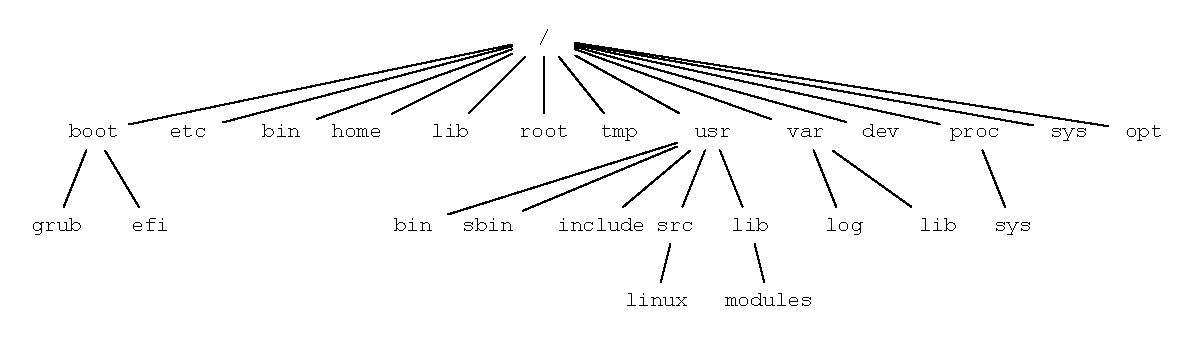
\includegraphics[scale=0.6]{figures/fs-tree.pdf}
	\centering
	\caption{The main directories in the root filesystem}
	\label{fig:fs-tree}
\end{figure}

\textbf{XXX---need to decide much of the tree I should describe}.

\begin{itemize}
	\item \cf{/bin} -- a symbolic link to \cf{/usr/bin} which contains almost 1500 general purpose commands such as \cf{ls(1)} 
		and \cf{mkdir(1)}.
	\item \cf{/etc} -- system-wide configuration files and system databases. It used to be the dumping ground for 
		everything else thus the name "etc" (etcetera). 
	\item \cf{/boot} -- the Linux kernel image, \cf{initrd} (initial RAM disk, GRUB configuration and anything else that
		is needed to bootstrap the system.
	\item \cf{/dev} -- all of the devices in the system. More specifically, these are special files that are used to access
		Linux devices attached to the system. 
	\item \cf{/home} -- home directories for users.
	\item \cf{/lib} -- a symbolic link to \cf{/usr/lib}. This directory shared libraries.
	\item \cf{/lib/modules} -- all of the compiled kernel modules are located under this directory. The filesystem modules 
		are located under \cf{/lib/modules/<kernel version>/kernel/fs}.
	\item \cf{/root} -- the home directory for \cf{root}. It's separated from \cf{/home} since user data is often kept on a 
		separate filesystem which is mounted later in the boot process. At various times it may be necessary to boot
		to single user mode and for root to be able to login and diagnose issues. This occurs before general filesystems
		are mounted.
	\item \cf{/usr/src/linux} -- the Linux headers are here by default but not the source code. Installing the kernel
		source code can be done using Linux distribution-specific commands or you can downloaded a kernel
		of your choice from \cf{www.kernel.org}.  To build a Linux kernel you don't need to put the source code here. You
		can build and install the kernel as a general user. This will be discussed more in chapter \ref{disk-fs}.
	\item \cf{/proc} -- there are many interesting bits of information in \cf{/proc} that are related to
		file access and filesystems. We'll be exploring these in section \ref{procfs}.
	\item \cf{/sbin} -- a symbolic link to \cf{/usr/sbin}, this directory contains programs used to boot and administer the 
		system. Programs here are not typically used by general users.
	\item \cf{/tmp} -- used for storing temporary files. Once upon a time, these files were cleared each time the system
		was rebooted. Now it is cleared after a predefined number of days which differs per Linux distribution. Just never 
		assume that any files you place here will still be there after the next reboot. The \cf{/var/tmp} directory is
		similar but has a longer retention period.
	\item \cf{/var/log} -- holds system log files.
	\item \cf{XXX} -- \textbf{more? check when reading back again}
\end{itemize}

%%%%%%%%%%%%%%%%%%%%%%%%%%%%%%%%%%%%%%%%%%%%%%%%%%%%%%%%%%%%

\section{How Simple it Used to be}

In early versions of UNIX as well as Linux, a disk partitioning was very simple. There was a bootstrap block and the UNIX  filesystem. To go back and see how UNIX handled the boot process back in 1975, you can get hold of John Lyons' "\textit{A Commentary on the 6th Edition UNIX Operating System}" online. The source code is available on github at: 

\begin{table}[h]
\begin{tabular}{lcl}
\parbox[r]{0.5in}{ 
\includegraphics[scale=0.15]{figures/url.png}} & \parbox[l]{0.1in}{\arabic{urls}} & \parbox[l]{3in}{\cf{https://tinyurl.com/u36a2a3a}}
\end{tabular}
\end{table}
\stepcounter{urls}
% https://github.com/memnoth/unix-v6

\noindent
In the top-level \cf{README.md} you will find a link to Lions' book. I remember when I first got hold of John Lions' book and seeing all of the UNIX source code at just over 11,000 lines of code. At the time I was working on getting the \cf{truss(1)} utility (UNIX equivalent of \cf{strace(1)} running on the SVR4 subsystem on the Chorus microkernel at the time. It was about the same amount of code. Gulp! How things were much simpler back then.

Bootstrap was very simple. The initial boot loader was located firmware. Its goal was to load block 0 which contained a larger boot program. This boot program looked for and loaded \cf{/unix} to which it passes control. The superblock of the root filesystem was always stored in block 1. \textbf{did they really not have mountable filesystems? I thought I saw mount in there somewhere? Check}

Additional filesystems could be mounted - \textbf{XXX---walk through the code and see how it worked}

% https://web.cs.wpi.edu/~rek/DCS/D04/UnixFileSystems.html - old fs layout - need more accurate info

%%%%%%%%%%%%%%%%%%%%%%%%%%%%%%%%%%%%%%%%%%%%%%%%%%%%%%%%%%%%

\section{Filesystems, Disks and Partitions}\label{partitions}

Things to cover:

\begin{itemize}
	\item physical vs logical block sizes
	\item maximum file and filesystem sizes and how fs block size affects this
	\item block allocation vs extents
	\item perhaps show old single, double and triple extents to show how things have changed
	\item full fsck vs journaling
	\item partition highlights before describing in more details in next sections
\end{itemize}

Filesystem on-disk structures have become considerable more complicated in the last thirty years compared to early days of UNIX and Linux.

%-----------------------------------------------------------------------------------------------------------------------------------------------------------------------

\subsection{Filesystem On-disk Structure}

Disks are partitioned using different partitioning schemes which will be described soon but generally speaking, there can be multiple partitions within a single disk and each partition can contain a filesystem that can be mounted separately onto a directory in the Linux file hierarchy. Figure \ref{fig:basic-disk-layout} shows the basic components of a traditional filesystem.

\begin{figure}[h]
	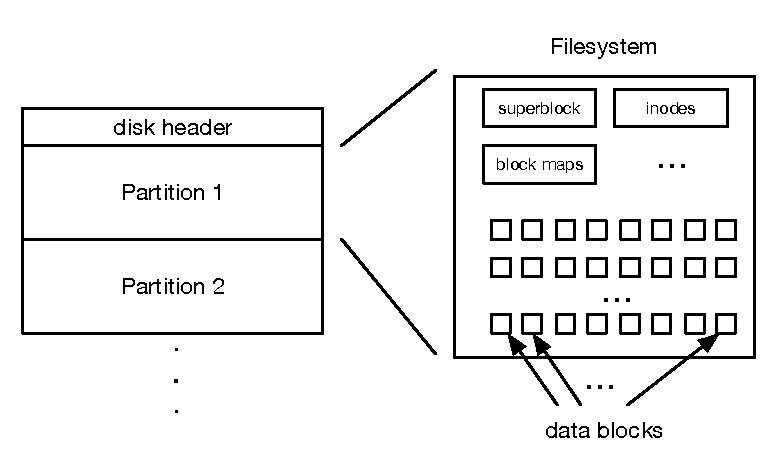
\includegraphics[scale=0.6]{figures/basic-disk-layout.pdf}
	\centering
	\caption{A disk partition with general filesystem disk structures}
	\label{fig:basic-disk-layout}
\end{figure}

\noindent
Todays filesystems are much more complicated and will described later in the book. However, this is the minimal set of data structures needed to create a fully functioning filesystem.

\begin{itemize}
	\item \textbf{superblock} -- the first structure that will be read from disk when the filesystem is mounted. It contains enough 
		information to locate the other structures needed to access files, allocate data blocks and so on. There may
		be multiple copies of the superblock to guard against disk errors. 
	\item \textbf{inode} -- a structure on disk that represents a file regardless of the file type. It contains file meta-data which 
		describes the file including type, size, owner and the location of the file's \textit{data blocks}. There may be
		a preallocated inode list or inodes may be allocated dynamically allowing for a larger number of files.
	\item \textbf{data blocks} -- contain actual data whether it be regular file data, directory entries or symbolic links.
	\item \textbf{block map} -- a data structure that indicates which blocks have been allocated. Data blocks are of fixed size and
		the size is chosen when the filesystem is created.
\end{itemize}

\noindent 
The filesystem on-disk structure has evolved considerably over time primarily to address resilience, performance, file and filesystem size but also to incorporate new features such as snapshots, file activity change logs and journaling capabilities.

%-----------------------------------------------------------------------------------------------------------------------------------------------------------------------

\subsection{Referencing Data Blocks From The Inode}

To help explain file and filesystem sizes and how they differ depending on the filesystem block size, consider figure \ref{fig:indirects} which shows the layout of a file in the ext2 filesystem. 

\begin{figure}[h]
	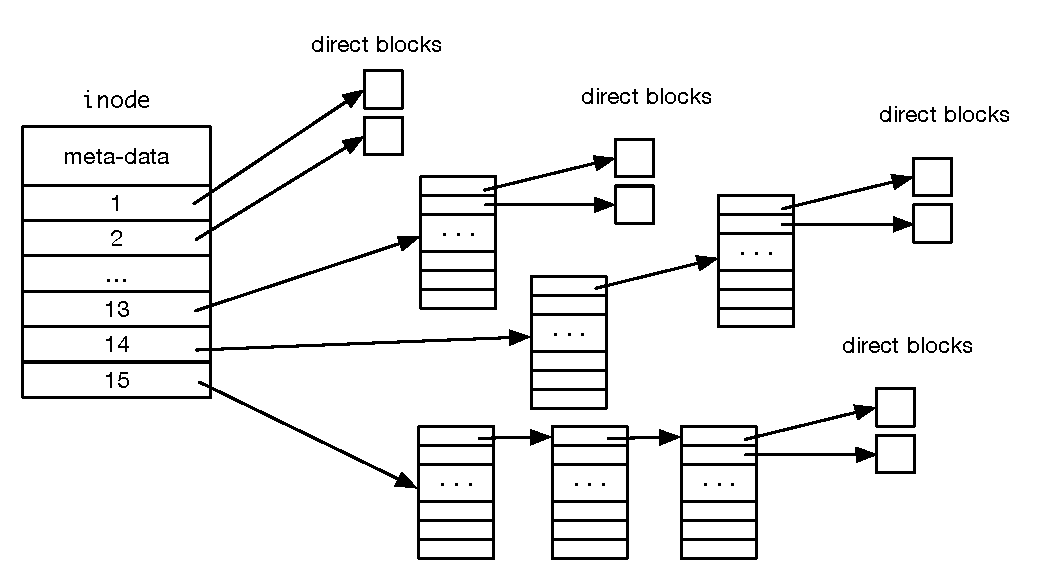
\includegraphics[scale=0.6]{figures/indirects.pdf}
	\centering
	\caption{The UFS on-disk structure for a file}
	\label{fig:indirects}
\end{figure}

\noindent
Inside the inode is meta-data about the file in addition to fifteen pointers that reference the file's data blocks either directly or indirectly. There are:

\begin{itemize}
	\item twelve direct pointers that points to blocks of actual data for the file.
	\item one single-indirect pointer that points to a block of pointers that then point to actual data blocks.
	\item one double-indirect pointer that points to a block of pointers that point to other blocks of pointers 
		that finally point to blocks of data for the file.
	\item one triple-indirect pointer that points to a block of pointers that point to other blocks of pointers 
		that point to other blocks of pointers that finally point to blocks of the file's data.
\end{itemize}

\noindent
The size of each block of data depends on the filesystem block size. Let's take ext4 as an example. It has four different filesystem block sizes that are specified when the filesystem is made. This means that each data block can range from 1 KB to 8 KB resulting in very different file sizes depending on the block size chosen as show in table \textbf{XXX---reverse direction and color}

\begin{table}
\centering
\begin{tabular}{|c|c|c|}
\hline
block size&maximum filesystem size&maximum file size\\
\hline
1 KiB&16 GB&4 TB\\
2 KiB&256 GB&8 TB\\
4 KiB&2 TB&16 TB\\
8 KiB&2 TB&32 TB\\
\hline
\end{tabular}
\end{table}

\noindent
xxx

%-----------------------------------------------------------------------------------------------------------------------------------------------------------------------

\subsection{Full Filesystem Check vs Journaling}

When a filesystem is mounted for read/write access, it is generally marked \textit{dirty} indicating that changes are occurring. This has traditionally been done by setting a flag in the superblock. When the filesystem is a unmounted it is marked \textit{clean}. If the system crashes between these two events, the filesystem could be in an inconsistent state. For example, when creating a file, there are several structures on disk that need to be modified. If the system crashes in the middle of these operations, the filesystem needs to undo those operations the operations that it performed to make the filesystem structurally intact again. To bring the filesystem back to being structurally intact, a \cf{fsck} (filesystem check) is needed. This is performed prior to the filesystem being mounted again, typically as part of the book process. This is a process that can take a very long time typically dependent on the number of files in the file system. Many hours there's not unlikely.

This is where \textit{filesystem journaling} comes into play. First introduced in the VERITAS VxFS filesystem and now available in several (name them???) Linux filesystems, journaling involves writing upcoming structural changes to an \textit{intent log} before changing the actual on-disk structures themselves. If the system crashes, log replay is performed which takes a very short amount of time. Journaling will be described in more detail in section TBD.

%-----------------------------------------------------------------------------------------------------------------------------------------------------------------------

\subsection{Disk Partitioning}

This is another topic to which a whole chapter could be dedicated but it really beyond the scope of this book. But partitioning affects many things from bootstrap to choosing how to layout filesystem. Whether using disks directly or using logical volume managers to manage the disks for you, it's important to spend some time explaining how disks are partitioned.

The two primary gains of GPT over MBR are:

\begin{enumerate}
	\item Large partitions, more that 2 TB
	\item Unlimited number of primary partitions
\end{enumerate}

%-----------------------------------------------------------------------------------------------------------------------------------------------------------------------

\subsection{The GPT Disk Format}

This section highlights the GPT format and shows how filesystems are stored within GPT partitions. A GPT-partitioned disk is shown in figure \ref{fig:gpt} with a hypothetical filesystem shown on partition 1. 

\begin{figure}
	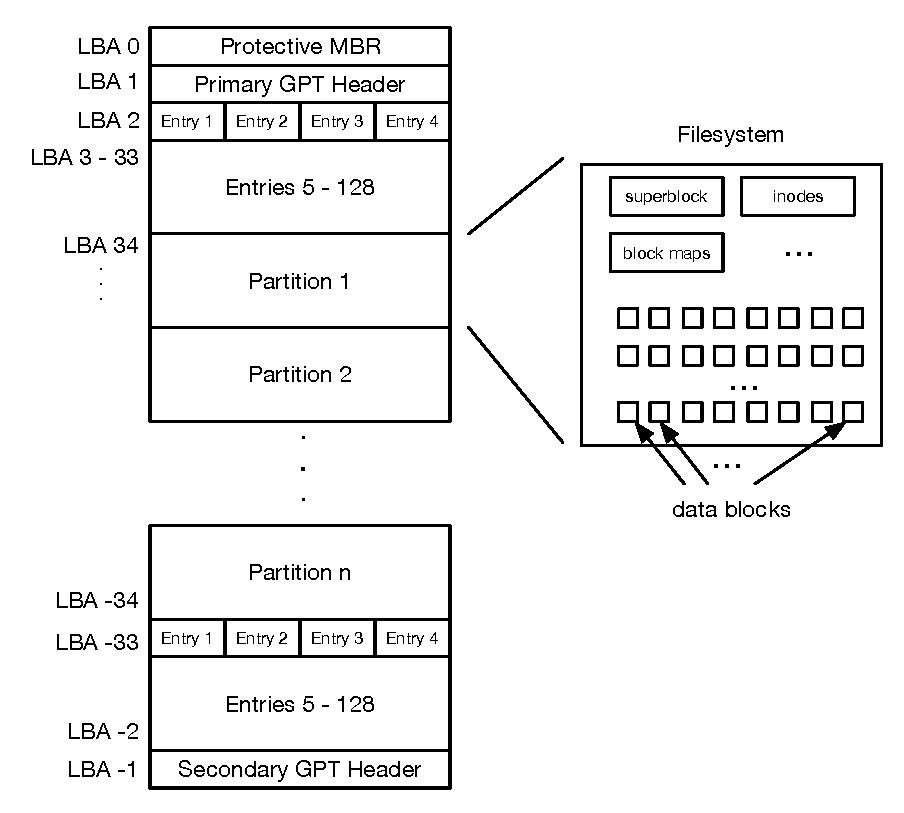
\includegraphics[scale=0.6]{figures/gpt.pdf}
	\centering
	\caption{GPT partitioned disk and filesystem within a partition}
	\label{fig:gpt}
\end{figure}

For each partition that contains a filesystem, the filesystem will \textit{manage} the layout of the partition. There will be filesystem meta-data which includes information about the filesystem itself (superblock), structures for allocated files (usually inode structures) and other information such as tracking data blocks which have been allocated. The meta-data only takes up a relatively small amount of space and the rest of the partition is open for storing file data. The exception to this is the RAM-based filesystems that have been used in Linux since early days (\textbf{XXX---day 1?}) which will be discussed in section \ref{ramfs}.

Some points to note about the figure:

\begin{itemize}
	\item LBA stands for Logical Block Addressing.  Each block is 512 bytes.
	\item There are two copies of the GPT header, one at the start of the disk and one in the last block (LBA - 1).
	\item The partition table starts at LBA 2 and there are up to 128 partitions. Each partition table entry is 128 bytes.
	\item \textit{Usable} partitions start with partition 1 and LBA 34. 
\end{itemize}

\noindent
blah 

%%%%%%%%%%%%%%%%%%%%%%%%%%%%%%%%%%%%%%%%%%%%%%%%%%%%%%%%%%%%

\subsection{Logical Volumes Managment}

For developmental or experimental purposes, you will likely only need one or two disk. On my Ubuntu VMs, I have one disk for Ubuntu itself and another small disk which I partition and use for storing filesystems that I'm developing or playing with. You can also create loopback devices and place filesystems on there.

In the real world, the amount of data that organizations need to store well exceeds the size of individual disks so managing hundreds, thousands or tens of thousands of individual disks makes no sense. This is where \textit{logical volume management} comes into play. Of course, most organizations will unlikely deal with disks themselves but rather get their storage management solutions from one of the many storage vendors on the market today. Each of these vendors will package many disks inside the storage arrays using logical volume manager technology for which some of the technology will be hidden from the customer.

Before working on the VERITAS filesystem VxFS, my first introduction to VERITAS came when I ported their volume manager VxVM to SVR4 UNIX running on the Chorus microkernel back in the early 1990s. VxVM was ported to many operating systems throughout the 90s, became a standard part of Microsoft Windows several during that time and my colleagues and friends ported it to Linux at the same time my team was porting VxFS to Linux.

%-----------------------------------------------------------------------------------------------------------------------------------------------------------------------

\subsection{Advantages of Logical Volume Management}

There are many advantages of logical volume management (LVM) and perhaps top of the list is ease of management. Rather than partitioning large numbers of disks and having to management them yourself, just give the disks to the volume manager and create new volumes as needed and not have them restricted by the size of the disk partitions.

Some have argued that LVM just adds another layer to the storage stack and has some performance overheard. However, the actual performance reduction is very minor and offset by the advantages that LVM offers. But as volumes are created and overlap on the underlying shared storage, fragmentation can become an issue leading to potential performance issues. These are all issues that the LVM vendors such as VERITAS addressed in their products.

Since this section is just highlighting the area of logical volume management, here are some of the major advantages:

\begin{itemize}
	\item Ease of management compared to handling large numbers of disks / partitions.
	\item Avoid the limits imposed by physical disk sizes / partitions.
	\item Increase or decrease the size of volumes and therefore the size of the filesystems that reside on them. For example,
		when extending the size of a filesystem, the operation can be done in five steps using Linux LVM. 
		Of course, if space is already available in the existing volume group, the first two steps can be omitted. 
	\begin{enumerate}
			\item Add new storage
			\item Create a new physical volume
			\item Extend the volume group to include the new physical volume
			\item Extend the Logical Volume 
			\item Extend the filesystem
		\end{enumerate}
	\item Performance gains through the use of \textit{striping}, where data is in a logical volume is spread across multiple
		devices and performance is increased since reads/writes happen in parallel.
	\item Redundancy through mirroring, where the same data is copied to two or more physical devices. If one of the devices
		dies or goes offline for some reason, the data on the other devices can still be accessed.
	\item Other RAID (Redundant Array of Inexpensive Disks) levels including RAID4 and RAID 5 which provide parity,
		a common way of detecting errors in a storage system. 
	\item Snapshots for backup purposes independent of the filesystem type. Not all filesystems support snapshot mechanisms.
\end{itemize}

\noindent 
Generally speaking, logical volume management allows users to build enterprise-level capabilities with inexpensive disks. Most modern storage systems have all of these capabilities built-in but come at additional cost.

%-----------------------------------------------------------------------------------------------------------------------------------------------------------------------

\subsection{Linux LVM}

Heinz Mauelshagen wrote the original LVM code back in 1998, taking its primary design guidelines from the HP-UX's volume manager, which was actually the VERITAS volume manager VxVM. I remember going to a small Linux conference in Frankfurt, Germany around that time that Heinz hosted. Version 1 of LVM was introduced into the 2.4 kernel series. LVM version 2 (or just LVM2) became available in kernel versions 2.6.9 and above.

Around this time, logical volume management was extremely popular with many organizations managing large numbers of disks which is problematic for many reasons. This popularity somewhat declined in subsequent years with newer storage arrays that had all of this functionality built-in. But in those cases, the logical volume management component simply shifted from the server or VM running Linux to the storage array itself. Take most IaaS (Infrastructure As A Service) solutions in the cloud. All of these capabilities are built in to the storage fabric and Linux just sees simple partitions. The same is true of most hypervisor solutions for which thin provisioning is an important capability but also hidden from the Linux operating system. Thing provisioning is a technique where storage blocks are only allocated as needed. It may look like you have 40 GB drive but if there is only 20 GB of data in used, only 20 GB of data is allocated from the underlying fabric.

Use of LVM still continues to this day. Some Linux distributions use LVM to configure the root device. For example, the Ubuntu VMs I am are partitioned as follows:

\begin{lstlisting}
$ [*\bfseries df -h*]
Filesystem                  Size Used Avail Use% Mounted on
tmpfs                       392M 1.2M  391M   1% /run
/dev/mapper/ubuntu--vg-...v  30G  21G  7.5G  74% /
tmpfs                       2.0G    0  2.0G   0% /dev/shm
tmpfs                       5.0M    0  5.0M   0% /run/lock
/dev/sda2                   2.0G 269M  1.6G  15% /boot
/dev/sda1                   1.1G 6.1M  1.1G   1% /boot/efi
tmpfs                       392M 4.0K  392M   1% /run/user/1000
\end{lstlisting}

\noindent
\textbf{XXX -- at some point, install other distros and see if they use LVM by default}

%-----------------------------------------------------------------------------------------------------------------------------------------------------------------------

\subsection{LVM Concepts}

LVM functions by layering abstractions on top of physical storage devices. The basic layers that LVM uses, starting with the most primitive, are shown in figure \ref{fig:LVM}:

\begin{figure}[h]
	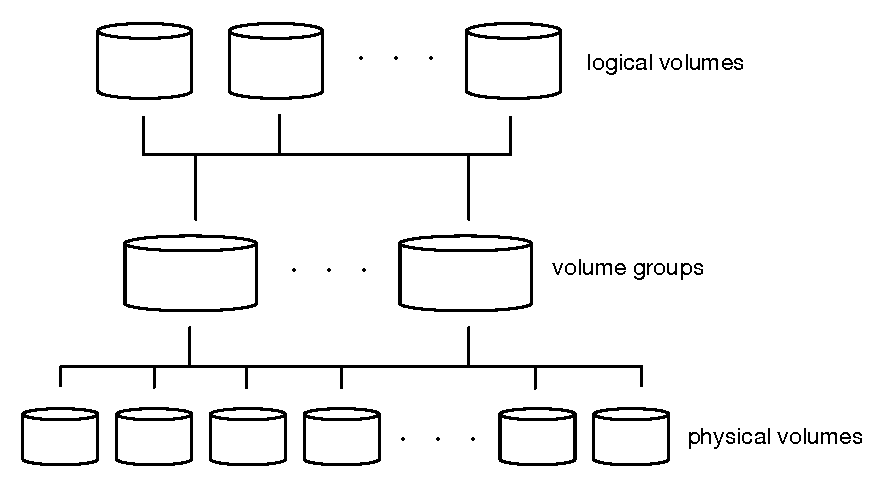
\includegraphics[scale=0.6]{figures/LVM.pdf}
	\centering
	\caption{LVM Architecture}
	\label{fig:LVM}
\end{figure}

\begin{itemize}
	\item \textbf{Physical Volumes} (PVs) -- LVM uses physical block devices such as hard disk drives, solid-state drives or 
		partitions. An LVM label is written near the start of the disk to correctly identify the device. This is particularly important
		when physical devices are removed/added since device names can change. The LVM utility prefix for physical volumes
		is \cf{pv}.
	\item \textbf{Volume Groups} (VGs) -- LVM combines physical volumes into storage pools called volume groups. You can
		think of them as very large disks. This concept was introduced in volume managers many years ago to allow for
		filesystems or raw volumes to be much bigger than the largest available disks at the time. The same is still true
		today. The LVM utility prefix for volume groups is \cf{vg}. 
	\item \textbf{Logical Volumes} (LVs) --  A volume group can be sliced up into any number of logical volumes. Logical volumes 
		are functionally equivalent to partitions on a physical disk in that you create a filesystem on top of a logical volume.
		However, they have much more flexibility. Logical volumes are the primary component that users and applications 
		will interact with. The LVM utility prefix for logical volumes is \cf{lg}. 
\end{itemize}

\noindent
Using the Ubuntu disk layout shown above, the following commands show the different LVM layers. First of all, here is the single physical volume which is constructed from a single disks \cf{/dev/sda3}:

\begin{lstlisting}   
$ [*\bfseries sudo pvdisplay*]
  --- Physical volume ---
  PV Name               /dev/sda3
  VG Name               ubuntu-vg
  PV Size               <60.95 GiB / not usable 3.00 MiB
  Allocatable           yes 
  PE Size               4.00 MiB
  Total PE              15602
  Free PE               7801
  Allocated PE          7801
  PV UUID               wpN3k3-OjXr-8FKN-CG0I-kf0B-hlK6-h0zXh9
\end{lstlisting}

\noindent
Next is the single volume group \cf{ubuntu-vg}:

\begin{lstlisting}   
$ [*\bfseries sudo vgdisplay*]
  --- Volume group ---
  VG Name               ubuntu-vg
  System ID             
  Format                lvm2
  Metadata Areas        1
  Metadata Sequence No  2
  VG Access             read/write
  VG Status             resizable
  MAX LV                0
  Cur LV                1
  Open LV               1
  Max PV                0
  Cur PV                1
  Act PV                1
  VG Size               <60.95 GiB
  PE Size               4.00 MiB
  Total PE              15602
  Alloc PE / Size       7801 / 30.47 GiB
  Free  PE / Size       7801 / 30.47 GiB
  VG UUID               CdWVPi-TAwA-7jtZ-iPFb-xq6k-ybeO-NKJNFY
\end{lstlisting}

\noindent
On top of this volume group there is a logical volume called \cf{ubuntu-lv}:

\begin{lstlisting}
$ [*\bfseries sudo lvdisplay*]
[sudo] password for spate: 
  --- Logical volume ---
  LV Path                /dev/ubuntu-vg/ubuntu-lv
  LV Name                ubuntu-lv
  VG Name                ubuntu-vg
  LV UUID                NXbsIa-999P-8QeO-aHJh-EdVU-jY2C-zOruGY
  LV Write Access        read/write
  LV Creation host, time ubuntu-server, 2023-04-19 09:13:27 +0000
  LV Status              available
  # open                 1
  LV Size                30.47 GiB
  Current LE             7801
  Segments               1
  Allocation             inherit
  Read ahead sectors     auto
  - currently set to     256
  Block device           253:0
\end{lstlisting}

\noindent
This is a very simple setup. If you want to play with LVM, you will need lots of disks and/or partitions. If you're operating in a virtualized world, that's very easy to do. You don't need to have large disks just to experiment.

%---------------------------------------------------------------------------------------------------------------------------------------------------------------------

\section{ZFS -- Builtin Volume Management}

The Z File System (ZFS) was created inside Sun Microsystems in 2001 by Bill Moore, Matthew Ahrens and Jeff Bonwick. It was designed to be the next generation file system for Sun Microsystems’ OpenSolaris following years of battles between Sun's UFS and the VERITAS filesystem VxFS. VxFS was much more feature rich and most of VERITAS' revenue came from Solaris, During this time Sun kept enhancing UFS mostly in the area of improving performance. This would be followed by an intense period at VERITAS to increase VxFS performance further.

In 2008, ZFS was ported to FreeBSD and we used it as part of the base OS at my second startup High Cloud Security. During the same year a port ZFS to Linux was initiated but has suffered due to the different licensing terms. ZFS is licensed under the Common Development and Distribution License (CDDL), which is incompatible with the GNU General Public License (GPL). Because of this, it cannot be included in the Linux kernel. To work around this problem ZFS if offered separately by some Linux distributions.

ZFS is a different filesystem altogether in that it includes builtin logical volume management.

Features include: \textbf{XXX -- need to look at this list, add more and get info from different sites}

\begin{itemize}
	\item Inline Data Compression -- xxx
	\item Send/Receive snapshots -- a \textit{snapshot} of a file system can be taken and this snapshot image can be sent 
		to a different server. This allows data from the original filesystem to be replicated for the purpose of 
		backing up data or enabling data migration to the cloud.
	\item Inline Data Deduplication -- xxx
	\item RAID-Z and Mirroring -- xx
	\item Hierarchical checksumming of all data and metadata -- xxx
	\item Automatic rollback of recent changes to the file system and data -- xxx
	\item Native handling of tiered storage and caching devices -- xxx
	\item Data integrity -- xxx
\end{itemize}

\noindent
Should you look at ZFS? The fact that it's not included directly in Linux distributions and may therefore have support issues, ZFS is a very feature-rich filesystem. Regardless of commercial use, it's worthy of study.

%%%%%%%%%%%%%%%%%%%%%%%%%%%%%%%%%%%%%%%%%%%%%%%%%%%%%%%%%%%%

\section{Filesystem Types Supported by Linux}

At the time of writing there are over 80 different filesystems supported by Linux. How many of them are actually used? 

It might be good to try and categorize them???

\begin{quote}
Wkipedia has a good page that i should cover - https://en.wikipedia.org/List\_of\_file\_systems
\end{quote}

\begin{itemize}
	\item Disk file systems
	\item File systems with built-in fault-tolerance
	\item File systems optimized for flash memory, solid state media
	\item Record-oriented file systems
	\item Shared-disk file systems
	\item Distributed file systems
	\item Distributed fault-tolerant file systems
	\item Distributed parallel file systems
	\item Distributed parallel fault-tolerant file systems
	\item Peer-to-peer file systems
	\item Special-purpose file systems
	\item Pseudo file systems
	\item Encrypted file systems --- this list excludes commercial solutions such as SecFS from 
		Thales (formerly Vormetric) and their FUSE-based encryption solution.
\end{itemize}

\noindent
In this book, we'll be covering pseudo filesystems as well as disk-based and FUSE-based filesystems. We'll also cover encrypted filesystems as part of looking at implementing a FUSE-based filesystem. 

%%%%%%%%%%%%%%%%%%%%%%%%%%%%%%%%%%%%%%%%%%%%%%%%%%%%%%%%%%%%

\section{How Many Filesystems are Actually Used?}

Although there are over 80 filesystems in the Linux kernel source and many FUSE and other filesystems elsewhere on the web, how many are actually used? Let's start with the root filesystem for the major Linux distributions today:

\begin{itemize}
	\item Ubuntu / Debian --- ext4
	\item Fedora --- btrfs 
	\item CentOS --- XFS
	\item RHEL --- XFS - was ext4 up to RHEL 6.0
	\item OpenSuSE --- btrfs
	\item SLES --- XFS
	\item Android --- ext4 or one of the flash-based filesystems such as YAFFS2. 
\end{itemize}

\noindent
Generally speaking, either \cf{ext4} or \cf{btrfs} are chosen as the default root filesystem apart from the server versions of Linux which use XFS. There are many opinions about whether \cf{btrfs} will replace \cf{ext4} in desktop or general non-server environments. It certainly has a lot more features but stability and performance are raised as concerns (at the time of writing). Generally speaking, I would advise to go with the default filesystem for a specific distribution unless you have specific needs or want to experiment with a different filesystem. The default filesystem will be the one most tested in the largest number of environments and situations. Since Ubuntu is the most widely used Linux distribution with the exception of mobile devices and Android devices either use ext4 or have been migrating towards \cf{ext4}, it could be argued that \cf{ext4} is the most widely used filesystem on Linux devices today.

On a default Ubuntu VM I have the following on the VMs I'm using when writing this book:

\begin{lstlisting}
$ [*\bfseries cat /proc/filesystems*]
nodev	sysfs
nodev	tmpfs
...
ext3
ext2
ext4
...
$ [*\bfseries cat /proc/filesystems | wc -l*]
33
$ [*\bfseries cat /proc/filesystems | grep nodev | wc -l*]
26
$ [*\bfseries mount | wc -l*]
32
\end{lstlisting}

\noindent
So interestingly enough, out of the 33 filesystem modules currently loaded, 26 of them are pseudo filesystems. By default, ext4 is the root filesystem on Ubuntu. Furthermore, running \cf{mount(1)}, there are 32 mounted filesystems. Here are the 7 that are displayed by \cf{df(1)}:

\begin{lstlisting}
$ [*\bfseries df -T*]
Filesystem  Type 1K-blocks    Used Available Use% Mounted on
tmpfs       tmpfs   400608    1340    399268   1% /run
/dev/map... ext4  39396672 1408380  25954836  31% /
tmpfs       tmpfs  2003028       0   2003028   0% /dev/shm                            
tmpfs       tmpfs     5120       0      5120   0% /run/lock
/dev/vda2   ext4   1992552  505692   1365620  28% /boot
/dev/vda1   vfat   1098628    5220   1093408   1% /boot/efi
tmpfs       tmpfs   400604       4    400600   1% /run/user/1000
\end{lstlisting}

\noindent
There are 3 FUSE filesystems that are registered which are not installed by default. They're available on my VM as I had been developing FUSE-based filesystems at the time of writing.

If you want the default filesystems that operating systems have used going back to 1968, the Wikipedia page (https://en.wikipedia.org/wiki/List\_of\_default\_file\_systems) provides an insight. It's not a very complete list as it excludes the various UNIX versions over the years as well as mainframe operating systems. For an historical perspective on Linux variants, it's more interesting. 

\noindent 
Another way to view mounted filesystems is to call the \cf{findmnt(8)} command, the output of which is shown in figure \ref{fig:findmnt}.

\begin{figure}
	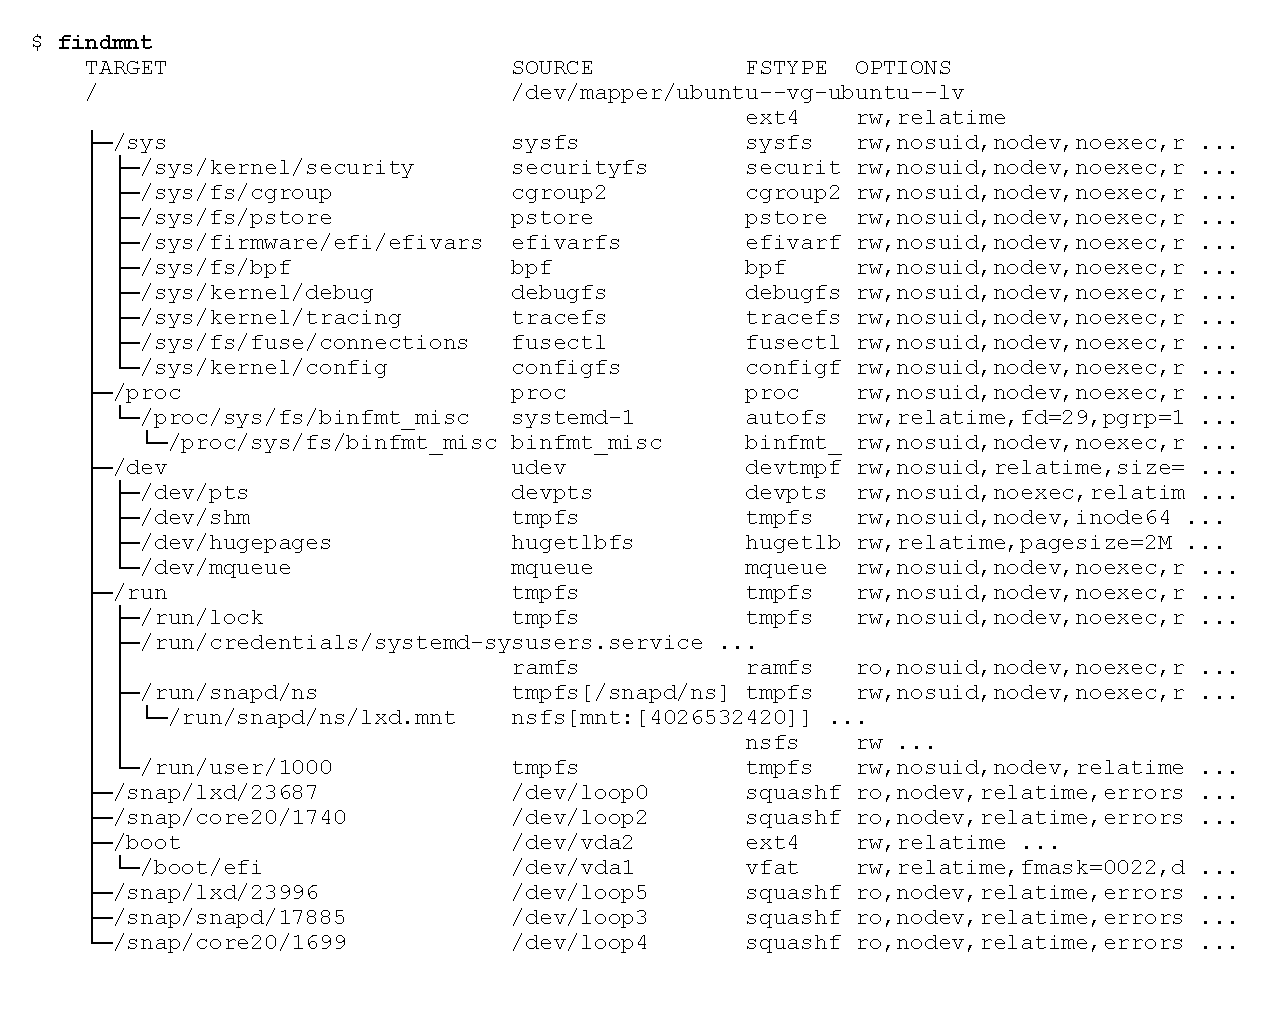
\includegraphics[scale=0.6]{figures/findmnt.pdf}
	\centering
	\caption{The \cf{findmnt(8)} command displays all mounted filesystems}
	\label{fig:findmnt}
\end{figure}

\noindent
You can also cat \cf{/proc/mounts} and get the same information but in a less pretty form.

%%%%%%%%%%%%%%%%%%%%%%%%%%%%%%%%%%%%%%%%%%%%%%%%%%%%%%%%%%%%

\section{Comparing the Main Filesystem Types}

% https://linuxiac.com/linux-file-system-types-explained-which-one-should-you-use/

Add some info about number of LOC for smallest, largest, most common etc

\begin{table}[h]
\begin{center}
\begin{tabular}{|p{0.2\textwidth}|m{0.4\textwidth}|}
\hline
\rowcolor[gray]{.93}\bf{Filesystem}&\bf{Lines Of Code (LOC)}\\
\hline
ext2 & 9,672\\
\hline
ext4 & 62,677\\
\hline
xfs & 70,520\\
\hline
btrfs & 146,306\\
\hline
\end{tabular}
\label{table:fs-loc}
\caption{\small Popular filesystems and their LOC in the kernel}
\end{center}
\end{table}

%-----------------------------------------------------------------------------------------------------------------------------------------------------------------------

\subsection{The ext2/3/4 Filesystems}

\textbf{XXX---still some plagerism particularly around bullet points}

The first Linux filesystem mirrored the filesystem structure from Andrew Tanenbaum's operating system MINIX. This had a number of limitations such as 14 character filenames and a maximum filesystem size of 64 MB. This filesystem was soon replaced with ext, the extended filesystem, which was added to Linux kernel version 0.96c in April 1992. It could handle file systems up to 2 GB and file names of up to 255 characters. But it had its own problems in that there was no support for separate timestamps for file access, inode modification, and data modification (atime, mtime and ctime).

To continue to make improvements, work on two new filesystems started in early 1993 for Linux kernel 0.99. These filesystems were xiafs developed by Frank Xia and the second extended file system (ext2) developed by R\'emy Card. Xiafs was still modeled around the MINIX filesystem while ext2 got its inspiration from the BSD filesystem UFS. Xiafs was less powerful and had less functionality than ext2 so over time, it was phased out. You won't find the source code in the Linux kernel any more while ext2 is still there (\cf{fs/ext2}).

The main features of ext2 or points to highlight are:

\begin{itemize}
	\item Block sizes of 1, 2, 4 and 8 KB.
	\item A maximum individual file size can be from 16 GB to 2 TB depending on the filesystem block size.
	\item A maximum file system size ranges from 4 TB to 32 TB depending on block size.
	\item Compression and decompression of files with the \cf{e2compr} patch.
	\item Since ext2 does not have journaling capabilities, if the system crashes, a full \cf{fsck} needs to be run. \textbf{TBC}
	\item On flash drives and USB drives, ext2 is recommended to reduce the overhead of journaling. \textbf{TBC}
\end{itemize}

\noindent
Ext3, or the third extended file system was introduced by Stephen Tweedie in 2001. It was merged into kernel version 2.4.15 in XXX. It had the following features:

\begin{itemize}
	\item Full filesystem journaling reducing the need for a full \cf{fsck} if the system crashes.
	\item Journaling has a dedicated area in the file system, where all the changes are tracked. When the system crashes, the 	\item possibility of file system corruption is less because of journaling.
	\item Maximum file size of 16 GB to 2 TB depending on block size.
	\item Filesystem between 2 TB to 32 TB depending on block size.
	\item You can convert a ext2 file system to ext3 file system directly (without backup/restore).
\end{itemize}

\noindent
There are three types of journaling available in ext3 file system.

\begin{itemize}
	\item Journal -- Metadata and content are saved in the journal.
	\item Ordered -- Only metadata is saved in the journal. Metadata are journaled only after writing the 
		content to disk. This is the default.
	\item Writeback -- Only metadata is saved in the journal. Metadata might be journaled either before or after 
		the content is written to the disk.
\end{itemize}

\noindent
The ext3 filesystem source code is no longer in the Linux kernel.

In June of 2006, Ted Ts'o, who was one of the the principal developers of ext3, announced ext4, the fourth extended file system. , The stable version was merged in the Linux kernel version 2.6.28 in October of 2008. He also stated that that although ext4 has improved features and is much faster than ext3, "\textit{it is not a major advance, it uses old technology, and is a stop-gap}". His belief is that btrfs is the better direction, because "\textit{it offers improvements in scalability, reliability, and ease of management}".

Ext4 has the following enhancements over ext3:

\begin{itemize}
	\item Supports huge individual file size and overall file system size.
	\item Maximum file size can be from 16 GB to 16 TB depending on the block size.
	\item Maximum file system size of 1 EB (exabyte). Note that 1 EB = 1024 PB (petabytes). 1 PB = 1024 TB (terabytes).
	\item Directories have a maximum of 64,000 subdirectories (this was increased from 32,000 in ext3)
	\item Several other new features are introduced in ext4: multi-block allocation, delayed allocation, 
		journal checksum. fast fsck, etc. All you need to know is that these new features have improved the 
		performance and reliability of the filesystem when compared to ext3.
	\item In ext4, you also have the option of turning the journaling feature “off”.
\end{itemize}

\noindent
XXX - what to write here depends on volume 1/2 vs a single book.

%-----------------------------------------------------------------------------------------------------------------------------------------------------------------------

\subsection{The XFS Filesystems}

XXX

Around the time we started the port of the VERITAS filesystem to Linux (late 1999), SGI were about to start porting their filesystem XFS. Soon after, both companies put out a press statement stating that the two companies had a joint project to bring a new, journaling filesystem to Linux. Since I was leading the effort at VERITAS I was surprised to see this news since I knew nothing of it. We quickly arranged a meeting between the two engineering teams (we were less than a mile apart) and all surprised that none of us ever knew anything about the press release. A quick marketing effort for some reason that none of us ever understood but we did stay in touch and shared our own experiences of porting what were likely, the two most feature rich commercial filesystems of the day.

\begin{itemize}
	\item Journaling -- 
	\item Allocation groups -- 
	\item Extent-based allocation -- 
	\item Striped allocation -- 
	\item A wide variety of block sizes -- from 512 bytes and 64 KB XXX
	\item Delayed allocation -- 
	\item Extended attributes - multiple data streams for files - hmm!
	\item Snapshots -- 
	\item On-line filesystem grow -- 
\end{itemize}

\noindent
XXX

%-----------------------------------------------------------------------------------------------------------------------------------------------------------------------

\subsection{The btrfs Filesystems}

% https://www.geeksforgeeks.org/how-to-create-btrfs-filesystem-in-linux-and-its-features/

Btrfs development began at Oracle in 2007. Btrfs is the next-generation general-purpose Linux file system that offers unique features like advanced integrated device management, scalability, and reliability. It is licensed under the GPL and open for contribution from anyone. There are different ways to pronounce the filesystem, including "Better FS”, “B-tree FS” and “Butter FS". Or just spell it out letter by letter. It was merged into the mainline Linux kernel in 2009 and first appeared in the Linux 2.6.29 release.

Goals

\begin{quote}
\textit{to let [Linux] scale for the storage that will be available. Scaling is not just about addressing the storage but also means being able to administer and to manage it with a clean interface that lets people see what's being used and makes it more reliable.}
\end{quote}

Although btrfs was included as a "technology preview" in Red Hat Enterprise Linux versions 6 and 7, it was removed in RHEL 8 in 2018. However, Fedora continued to offer it. \textbf{XXX---need to follow up on this one}. Looks like Red Hat have several XFS developers working for them.

The main features of btrfs are:

\begin{enumerate}
	\item \textbf{Extent-based allocation} -- earlier in the chapter, traditional disk layouts were described where blocks 
		are allocated to a file as direct, indirect, double indirect or triple indirects. In past times when files were not the 
		huge sizes that can be seen today, this was adequate. Extent based allocation was introduced in VxFS and XFS.
		In this scheme, variable size extents are allocated to a file. Take the case of a database. If the size of the database
		is known upfront and, let's say, that it's going to be 1 TB, why not have a single extent of 1 TB. This simplifies the
		inode structure and guarantees that all the data is contiguous on disk getting the best in terms of performance.
	\item Checksums -- 
	\item Cloning -- 
	\item Self-healing -- 
	\item Deduplication -- 
	\item Compression -- 
	\item Snapshots -- XXX. There is an example of using btrfs snapshots in section \ref{btrfs-snapshots}.
	\item Quota groups --
	\item File cloning -- 
	\item In-place conversation --
	\item Union mounting / seed devices -- 
	\item Online defragmentation, volume growth, and shrinking -- 
	\item Ability to handle swap files and swap partitions --
\end{enumerate}

\noindent
xxx

\subsection{The Flash??? Filesystems}

XXX - yaffs2 etc? F2FS 

\subsection{Stratis - RHEL???}

Wrong place but need to cover it.

% https://access.redhat.com/discussions/3138231 - see comments

%%%%%%%%%%%%%%%%%%%%%%%%%%%%%%%%%%%%%%%%%%%%%%%%%%%%%%%%%%%%

\section{Kernel or Userspace?}

Implementing a kernel-based filesystem is not trivial. I've worked on filesystem development for UNIX SVR3, SVR4, SCO UNIX, HP-UX, UnixWare, Solaris, Linux and various UNIX subsystems built on top of the Chorus microkernel. I actually started my filesystem career working on RFS back in the late 1980s. Debugging filesystems in the kernel is not easy. I've enjoyed using source level debuggers on HP-UX and Linux (through \cf{gdb} / \cf{kgdb}) but have also been stuck working at assembler level a lot and even had the pleasure (pain?) of working on debugging Solaris filesystems in \cf{adb} (yes, all in assembler) on Sparc systems with their peculiar register windows and lack of developer trust in arguments displayed in a stack trace.

But if you want performance, you'll be using one of the disk-based filesystems running on top of a high-performance storage system. \textbf{raw vs XXX}

In many cases, performance is not critical. For example, for personal use, I keep all of my source code files on my Mac where they're backed up and use SSHFS, which is a user-space filesystem developed using FUSE. Performance is not critical and usability wins the day. \textbf{XXX---expand on this}.

\textbf{does this section really belong here?}

%%%%%%%%%%%%%%%%%%%%%%%%%%%%%%%%%%%%%%%%%%%%%%%%%%%%%%%%%%%%

\section{Pseudo Filesystems}

A filesystem comprises a number of files which can be different types such as regular files or directories. In most cases, we deal with physical filesystems where these files are permanently stored. A pseudo filesystem on the other hand does not contain permanent storage. They are constructed as the kernel initializes and destroyed when the kernel shuts down.

The 3 well-known pseudo filesystems on Linux are proc (also called the /proc filesystem) which is mounted on \cf{/proc}, ramfs (\textbf{image when loading - come back to this}) and the sysfs filesystem which is mounted on \cf{/sys}. 

devfs), or a middle point such as Linux devtmpfs ???

Which pseudo filesystems are generally used? In my Ubuntu server VM, I've installed FUSE (which has 3 registered filesystems) but in addition to these, there are another 23 registered pseudo filesystems:

\begin{lstlisting}
$ [*\bfseries cat /proc/filesystems | grep nodev*]
nodev   sysfs
nodev   tmpfs
nodev   bdev
nodev   proc
nodev   cgroup
nodev   cgroup2
nodev   cpuset
nodev   devtmpfs
nodev   configfs
nodev   debugfs
nodev   tracefs
nodev   securityfs
nodev   sockfs
nodev   bpf
nodev   pipefs
nodev   ramfs
nodev   hugetlbfs
nodev   devpts
nodev   ecryptfs
nodev   fuse
nodev   fusectl
nodev   efivarfs
nodev   mqueue
nodev   pstore
nodev   autofs
nodev   binfmt_misc
\end{lstlisting}

\noindent
\textbf{XXX---need to think about how much to say here or whether we cover 1 or more in the kernel chapter}

%-----------------------------------------------------------------------------------------------------------------------------------------------------------------------

\subsection{The proc Filesystem}\label{procfs}

One filesystem that we will explore here is the proc pseudo filesystem (mounted on \cf{/proc} and also sometimes called the /proc filesystem) which contains a wealth of information about running process and a lot more information about the running system. It also provides the means through which different kernel parameters can be changed. There are close to 17,000 lines of code in the proc filesystem.

\begin{figure}[h]
	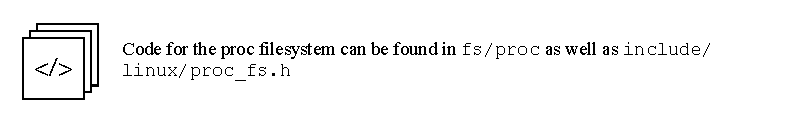
\includegraphics[scale=0.95]{src-xref/procfs.pdf}
\end{figure}

The proc filesystem can be traced all the way back to UNIX 8th Edition and was first described in the 1984 USENIX paper "\textit{Processes as Files}":

\begin{table}[h]
\begin{tabular}{lcl}
\parbox[r]{0.5in}{ 
\includegraphics[scale=0.15]{figures/url.png}} & \parbox[l]{0.1in}{\arabic{urls}} & \parbox[l]{3in}{\cf{https://tinyurl.com/mvmb6nnj}}
\end{tabular}
\end{table}
\stepcounter{urls}
% https://lucasvr.gobolinux.org/etc/Killian84-Procfs-USENIX.pdf

The proc filesystem was then further developed as a collaboration between Sun Microsystems and AT\&T Bell Labs in the early 1990s for SVR4 UNIX and Solaris . Oddly enough, it actually began as a replacement for the \cf{ptrace(2)} system call which was the primary interface for debugging applications. Another goal was to replace ioctl(2) calls with standard \cf{read(2)} and \cf{write(2)} system calls which are better suited to network access. Commands such as \cf{ps(1)} and \cf{truss(1)} (UNIX version of \cf{strace(1)} were rewritten to use \cf{/proc}. I fully recommending reading the old USENIX paper.

\begin{table}[h]
\begin{tabular}{lcl}
\parbox[r]{0.5in}{ 
\includegraphics[scale=0.15]{figures/url.png}} & \parbox[l]{0.1in}{\arabic{urls}} & \parbox[l]{3in}{\cf{https://tinyurl.com/4wpmth6u}}
\end{tabular}
\end{table}
\stepcounter{urls}
% https://www.usenix.org/sites/default/files/usenix_winter91_faulkner.pdf

The proc filesystem was introduced in to Linux in 1992. Processes are described by looking at \cf{/proc/PID} where \cf{PID} is the process ID. FIgure \ref{fig:ls-proc} shows what's in \cf{proc} on my Ubuntu VM. As you can see, there is a lot more  in there other than just process-related information.

\begin{figure}
	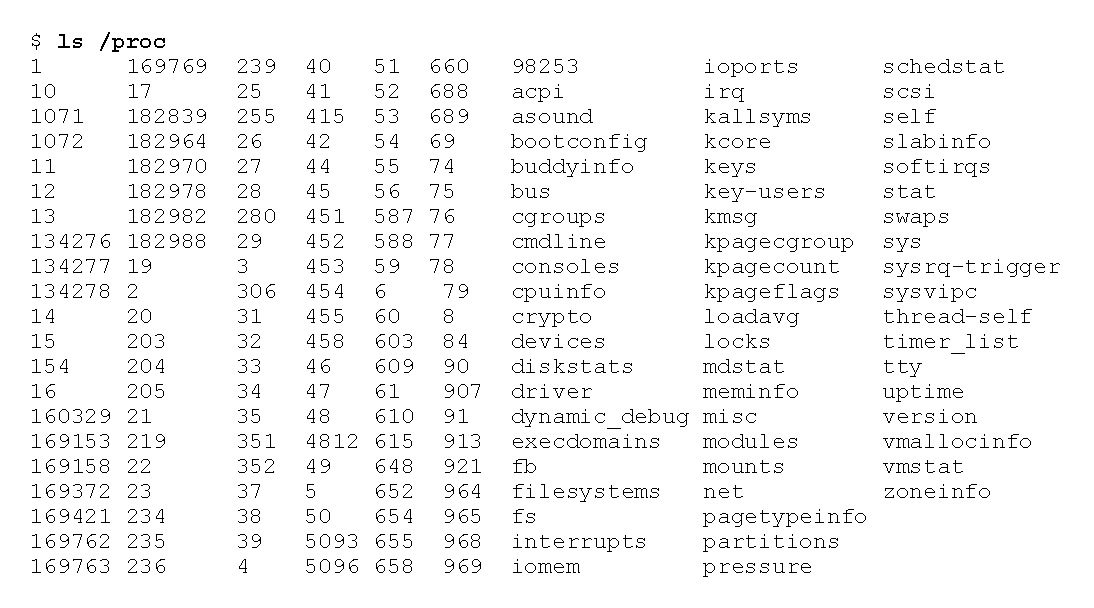
\includegraphics[scale=0.68]{figures/ls-proc.pdf}
	\centering
	\caption{The contents of \cf{/proc} on Ubuntu}
	\label{fig:ls-proc}
\end{figure}

For a process to get information about itself it can look under \cf{/proc/self}. Let's do a little exploring from the shell.

\begin{lstlisting}
$ [*\bfseries cd /proc/self*]
$ [*\bfseries cat cmdline*]
-bash           # actually doesn't add a newline
$ [*\bfseries ls -l exe*]
lrwxrwxrwx 1 spate spate 0 Nov 29 06:20 exe -> /usr/bin/bash
\end{lstlisting}

Need to look at following for /proc/self/fds/255 - %https://askubuntu.com/questions/866712/what-are-these-auxiliary-file-descriptors/866722#866722

Good site - %https://tldp.org/LDP/Linux-Filesystem-Hierarchy/html/proc.html

%-----------------------------------------------------------------------------------------------------------------------------------------------------------------------

\subsection{The Ramfs Filesystem}\label{ramfs}

One pseudo filesystem that is always used and part of the boot process is Ramfs, a RAM-based filesystem. XXX need to get info on how it's built.

The code for Ramfs is very small at only just over 600 lines of code.  Since it's so small, the ramfs module is always loaded

\begin{table}[h]
\begin{tabular}{ll}
\parbox[l]{0.6in}{
\includegraphics[scale=0.8]{figures/src-xref.pdf}} & \parbox[l]{4in}{\small{All of the Ramfs code can be found in \cf{fs/ramfs}.}}
\end{tabular}
\end{table}

\noindent
There really isn't a lot too the code and the filesystem relies mostly on generic VFS-level operations. We'll describe these in detail in section \ref{vfs}.

% https://www.kernel.org/doc/Documentation/filesystems/ramfs-rootfs-initramfs.txt - good doc

Ramfs is only used as part of the boot process (really?). To create the older RAM-based filesystem,  a pseudo block device (just allocate a virtually contiguous area of memory) was created on which to place the filesystem and a filesystem was placed in it (usually ext2). This imposed size limits which could be problematic at times and resulting in wasting time copying data to and from this \textit{device} into the page cache plus using part of the device for ext2-specific data such as inodes and block maps. The pseudo device was removed a long time ago which simplified many things including the fixed space issue and a switch was made to the new ramfs filesystem. But this also potentially created other problems in that since it would be possible to fill up memory as more and more files were created. The first step to avoid this was to restrict it to superuser access. 

%-----------------------------------------------------------------------------------------------------------------------------------------------------------------------

\subsection{The tmpfs Filesystem}

% start with Documentation/filesystems/tmpfs.rst

See rest of chapter - it's used everywhere

%-----------------------------------------------------------------------------------------------------------------------------------------------------------------------

\subsection{The pipe Filesystem}\label{pipefs}

fs/pipe.c calls register\_filesystem().

%-----------------------------------------------------------------------------------------------------------------------------------------------------------------------

\subsection{The AuFS Filesystem}

\textbf{While most Live CD linux distributions used Aufs as of November 2016, Slackware used overlayfs for its live CD} - so is it relevant or not?

%-----------------------------------------------------------------------------------------------------------------------------------------------------------------------

\subsection{The OverlayFS Filesystem}

xxx

%%%%%%%%%%%%%%%%%%%%%%%%%%%%%%%%%%%%%%%%%%%%%%%%%%%%%%%%%%%%

\section{FUSE-based Filesystems}

Linux provides a framework called FUSE (FileSystem in User spacE) that allows filesystems to be developed in user space, a much simpler process than developing a kernel-based filesystem. Although performance has been an issue over the years, there are have been many improvements over the years and at the time of writing, there are some eBPF enhancements which could also increase performance. 

Commercial vendors have a hard time implementing kernel-based filesystems due to lack of access to all kernel symbols (functions etc) as well as having to keep up with kernel updates. Either the commercial filesystem needs to be recompiled for each new kernel version or filesystem modules are force-loaded assuming testing reveals no issues. The latter works for minor Linux kernel updates. But there has been success in developing FUSE-based filesystems. One such example is the Thales CipherTrust Transparent Encryption UserSpace which provides encryption and access controls. This has proven to be acceptable in a number of customer environments, typically where performance is not critical.

Figure \ref{fig:fuse-fs-chap} shows components when using a FUSE-based filesystem.

\begin{figure}
	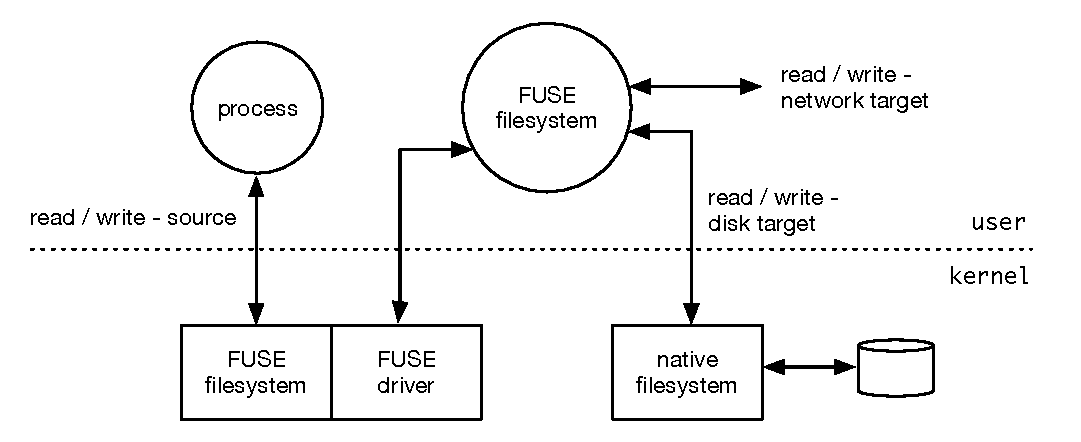
\includegraphics[scale=0.6]{figures/fuse-fs-chap.pdf}
	\centering
	\caption{FUSE filesystems allow development in user-space}
	\label{fig:fuse-fs-chap}
\end{figure}

Applications access files as normal unaware that they are using a FUSE filesystem. Inside the kernel, the FUSE kernel components route file operations up into user-space where they are handled by a FUSE library and the FUSE filesystem component which then routes these calls either back into the kernel to different part of the filesystem or over the network to a remote service. 

cover mount options a little

There are a lot of FUSE-based filesystems. The FUSE Wikipedia page has a large list. We'll describe a few here and then give an example of using one in particular.

\begin{itemize}
	\item s3fs --- the ability to mount an AWS S3 bucket and view the objects as files
	\item EncFS --- a filesystem that encrypts files and contents. Security concerns were raised about
		EncFS and there was rumored to be a newer version which would fix these concerns. That hasn't
		yet happened.
	\item SSHFS --- access to a remote filesystem through use of SSH.
	\item WikipediaFS --- the ability to view Wikipedia pages as if there were local files. It has since
		been deprecated.
\end{itemize}

In section \ref{fuse-chapter} I'll be showing you how to develop two FUSE-based filesystems. The first will just "pass-through" operations whereby part of the file hierarchy will be visible through another directory. Files can be created, deleted and accessed as normal. The second filesystem will add encryption for file names and contents.

%------------------------------------------------------------------------------------------------------------------------------------------------------------------------

\subsection{Demonstrating the SSHFS FUSE Filesystem}\label{ssh-fuse}

I wanted to demonstrate the WikipediaFS filesystem but found that it was deprecated many years ago. The same seems to be somewhat true of SSHFS. The github page indicates that the project is no longer maintained or developed although there have been changes within the last year. The repository has been archived so it's now read-only. It's also available to be installed, at least on Ubuntu. So let's give it a try. First, it needs to be installed:

\begin{lstlisting}
$ [*\bfseries sudo apt install sshfs*]
\end{lstlisting}

\noindent
Next, we'll create a local directory on to which we will mount the remote directory. We run \cf{mount(1)} to verify that it's mounted. Note that the \cf{sshfs} command backgrounds itself.

\begin{lstlisting}
$ [*\bfseries mkdir remote*]
$ [*\bfseries sshfs spate@192.168.4.21:~/src/spfs remote*]
(spate@192.168.4.21) Password:
$ [*\bfseries mount | grep remote*]
spate@192.168.4.21:/Users/spate/src/spfs on /home/spate/remote \
type fuse.sshfs (rw,nosuid,nodev,relatime,user_id=1000,\
group_id=1000)
\end{lstlisting}

\noindent
At this point, all files are visible just as if they were local:

\begin{lstlisting}
$ [*\bfseries ls remote*]
cmds  kern  LICENSE  README  test
$ [*\bfseries ls remote/kern*]
add_stuff  dir.c     Makefile    sp_dir.c   spfs.h  sp_ioctl.c
dir2.c     fillfs.c  sp_alloc.c  sp_file.c  sp_inode.c
\end{lstlisting}

\noindent
You can move around the directory structures, create, remove and read/write files. When you want to unmount the filesystem simply run:

\begin{lstlisting}
$ [*\bfseries fusermount -u remote*]
\end{lstlisting}

\noindent
I spend a lot of time running scripts to sync files between my Mac and my Linux VMs. This looks like a much easier method so happy I gave it a try.

%%%%%%%%%%%%%%%%%%%%%%%%%%%%%%%%%%%%%%%%%%%%%%%%%%%%%%%%%%%%%%%

\section{Physical Filesystems and Partitioning}\label{mkfs-examples}

- grub
- fdisk or whatever is used now
- limitations of disk sizes - relevant any more
- raw vs block devices

\textbf{XXX---example with partitioning and multiple filesystems on same disk / different partitions}

I've partitioned my 1 GB virtual disk into two partitions using \cf{fdisk(8)} so now I have two partitions:

\begin{lstlisting}
# [*\bfseries ls /dev/sd??*]
/dev/sda1  /dev/sda2
\end{lstlisting}

\noindent
And now I can create a filesystem on each partition, mount each filesystem and copy some files into both:

\begin{lstlisting}
# [*\bfseries mkfs -t ext4 /dev/sda1*]
...
# [*\bfseries mkfs -t btrfs /dev/sda2*]
...
# [*\bfseries mount -t ext4 /dev/sda1 /mnt1*]
# [*\bfseries mount -t btrfs /dev/sda2 /mnt2*]
# [*\bfseries cp /etc/* /mnt1 2> /dev/null*]
# [*\bfseries cp /etc/* /mnt2 2> /dev/null*]
# [*\bfseries df -h | grep mnt*]
/dev/sda1        703M  552K  651M   1% /mnt1
/dev/sda2        291M  3.9M  210M   2% /mnt2
# [*\bfseries df -h*]
Filesystem       Size  [*\bfseries Used*] Avail Use% Mounted on
...
/dev/sda1        703M  [*\bfseries 552K*]  651M   1% /mnt1
/dev/sda2        291M  [*\bfseries 3.9M*]  210M   2% /mnt2
\end{lstlisting}

\noindent
Note that although we have copied the same amount of data into each filesystem, the btrfs filesystem has used a lot more space than ext4. Some filesystems use more space for meta-data and some filesystems allocated meta-data up front while others allocate it dynamically therefore usage varies depending on the filesystem type. With the size of today's disks, it's really not a big deal.

%%%%%%%%%%%%%%%%%%%%%%%%%%%%%%%%%%%%%%%%%%%%%%%%%%%%%%%%%%%%

\section{Linux Namespaces}

% https://docs.kernel.org/userspace-api/unshare.html - good doc about unshare(2) and kernel support

Linux \textit{namespaces} are a feature of the Linux kernel that allow for different types of process isolation. Linux partitions different kernel resources such that one group of processes sees one set of resources while another group of processes can see a different set of resources. Namespaces were introduced into the Linux kernel in 2002 with enhancements and extensions continuing over the next several years. Namespaces are a fundamental aspect of how containers are implemented in Linux.

Since Linux kernel version 5.6, there are now eight different kinds of namespaces. All but the MNT namespace are beyond the scope of this book.

\begin{itemize}
	\item \textbf{Mount (MNT)} -- a  list of mount points seen by the processes in this particular namespace. Filesystems can be 
		mounted and unmounted in a mount namespace without impact on the main Linux filesystem.
	\item \textbf{Process ID (PID)} -- this namespace has a different set of PIDs from other namespaces. PID namespaces 
		are nested such that if a process is created it will have a one PID in the current namespace and a different PID
		in all namespaces above it up to the initial PID namespace. The first process created in any new PID namespace 
		is assigned the process ID number 1.
	\item \textbf{Network (NET)} -- 
	\item \textbf{Inter-process Communication IPC)} -- 
	\item \textbf{UTS} -- 
	\item \textbf{User ID (USER)} -- 
	\item \textbf{Control group (CGROUP) Namespace} -- 
	\item \textbf{Time Namespace} -- 
\end{itemize}

\noindent
The MNT namespace is particularly relevant to filesystem access and you will see references to it through various parts of the filesystem code. It will be explained in the next section.

A Linux system starts out with a single namespace of each type and is used by all processes. Processes can create additional namespaces and/or join different namespaces. Namespaces are a fundamental aspect of containers on Linux and will be described in the next section.

Mount namespaces provide isolation regarding the list of mounts as seen by the process/tasks in each namespace. This ensures that different processes/tasks that belong to different mount namespaces will see distinct directories hierarchies.

Namespaces are documented in the \cf{unshare(1)} command and \cf{clone(2)} system call manpages. For an overview see the \cf{mount\_namespaces(7)} manpage.

% https://itnext.io/chroot-cgroups-and-namespaces-an-overview-37124d995e3d - chroot, cgroups and namespaces

More notes:

\begin{enumerate}
	\item Namespaces are often used when untrusted code has to be executed on a given machine without compromising 
		the host OS.
	\item on process namespaces - All ‘ps’-like commands use the virtual procfs file system mount to deliver their functionalities.
	\item Linux processes form a single hierarchy, with all processes rooting at init. Usually privileged processes in this tree can trace or kill other processes.Linux namespace enables us to have many hierarchies of processes with their own “subtrees” such that processes in one subtree cant access or even know of those in another.
	\item If we create a PID namespace and run a process in it, that first process becomes PID 1 in that namespace. 
	\item But this only means that the processes within the new namespace can not see parent process but the parent process namespace can see the child namespace. And the processes within new namespace now have 2 PIDs: one for new namespace and one for global namespace.
	\item Linux kernel now tracks process’s PIDs using upid structure instead of a single pid value. The upid structure tells about the pid and the namespaces where that pid is valid.
	\item There are new APIs - clone(), setns() and unshare() - need to look at them.
The above "flags" (CLONE\_NEWNS, CLONE\_NEWUSER etc) are passed to clone() to create that type of namespace.
\end{enumerate}

%--------------------------------------------------------------------------------------------------------------------------------------------------------------------

\subsection{Shared Subtrees}

Damn! This stuff is complicated!

% https://www.kernel.org/doc/Documentation/filesystems/sharedsubtree.txt - shared subtrees - relevant?
% https://lwn.net/Articles/689856/ - Mount namespaces and shared subtrees

\begin{itemize}
	\item \cf{MS\_SHARED} --  This mount point shares mount and unmount events with other mount points that 
		are members of its “peer group”. When a mount point is added or removed under this mount point, 
		this change will propagate to the peer group, so that the mount or unmount will also take place under 
		each of the peer mount points. Propagation also occurs in the reverse direction, so that mount and 
		unmount events on a peer mount will also propagate to this mount point.
	\item \cf{MS\_PRIVATE} -- This is the converse of a shared mount point. The mount point does not propagate 
		events to any peers, and does not receive propagation events from any peers.
	\item \cf{MS\_SLAVE} -- This propagation type sits midway between shared and private. A slave mount has a 
		master — a shared peer group whose members propagate mount and unmount events to the slave mount. 
		However, the slave mount does not propagate events to the master peer group.
	\item \cf{MS\_UNBINDABLE} -- Does not receive or forward any propagation events and cannot be bind mounted.
\end{itemize}

\noindent
xxx
	
%--------------------------------------------------------------------------------------------------------------------------------------------------------------------

\subsection{Root and \cf{chroot} Environments}

%<<<
In a Unix-like OS, root directory(/) is the top directory. root file system sits on the same disk partition where root directory is located. And it is on top of this root file system that all other file systems are mounted. All file system entries branch out of this root. This is the system’s actual root.

But each process has its own idea of what the root directory is. By default, it is actual system root but we can change this by using chroot() system call. We can have a different root so that we can create a separate environment to run so that it becomes easier to run and debug the process. Or it may also be to use legacy dependencies and libraries for the process.

It may appear that by separating a process using chroot()we ensure security by restricting the process not to access outside its environment. But in reality that is not very true. chroot() simply modifies pathname lookups for a process and its children , prepending the new root path to any name starting with /.Current directory is not modified and relative paths can refer any locations outside of new root.
%>>>

Yeah so can you chroot when logging in to solve this???

\subsection{Linux cgroups to Isolate and Manage Resources}

%<<<
Control groups(cgroups) is a Linux kernel feature which limits, isolates and measures resource usage of a group of processes. Resources quotas for memory, CPU, network and IO can be set. These were made part of Linux kernel in Linux 2.6.24.
%>>>

sound great for virtualization - yes. what we want is:

%<<<
Suppose we have an application we want to isolate usage for. Lets call it A1. Lets call rest of system as S. We will create a control group and assign resource limits on it: say 3GB of memory limit and 70\% of CPU. Then we can add requisite application’s process id to the group and application resource usage now is throttled. Though the application may exceed the limits in normal scenarios, it will be throttled back to pre set limits in case system is facing resource crunch. This makes even more sense when we are handling many VMs running on a machine-have a cgroup for VMs and throttle them individually to a set limit when resource contention happens.
%>>>

to install:

sudo apt-get install cgroup-bin cgroup-lite cgroup-tools cgroupfs-mount libcgroup1

%<<<
We can see a /cgroup directory created: this is used as mount point for cgroup virtual filesystems. etc/cgconfig.conf file gives info on what all mounts to expect. All controllers are mounted to /cgroup followed by controller name. eg/- /cgroup/memory.To mount the requisite controllers, run sudo service cgconfig restart .Following this we see directories in /cgroup, each of which can be used to manage a cgroup subsystem.
%>>>

https://itnext.io/chroot-cgroups-and-namespaces-an-overview-37124d995e3d - gives an example of using cgroups with a process that allocates more memory than allowed and gets killed. OK, good so far.

%--------------------------------------------------------------------------------------------------------------------------------------------------------------------

\subsection{Mount Namespace Example}

It always helps to see things in practice. This example shows how to create mount namespaces and show how mounts are shared or not shared depending on how \textbf{XXX - TBD}

\begin{lstlisting}
$ [*\bfseries sudo unshare -m bash*]
# [*\bfseries mount -t tmpfs tmpfs /mnt*]
# [*\bfseries touch /mnt/file*]
\end{lstlisting}

\noindent
in another terminal:

\begin{lstlisting}
$ [*\bfseries ls /mnt*]
lost+found/
\end{lstlisting}

\noindent
the newly created file is not visible. Further, once you exit the namespace, the file and mount point are no longer visible.

But this doesn't work for disk-based mount points. even if you create two namespaces and then mount -t spfs in one namespace, it's visible everywhere. XXX - Must be doing something wrong or just not understanding this properly.

Inside \cf{proc} you can see the mounting points visible for a specific process through the following paths:

\begin{enumerate}
	\item \cf{/proc/[PID]/mounts}
	\item \cf{/proc/[PID]/mountinfo}
	\item \cf{/proc/[PID]/mountstats}
\end{enumerate}

%--------------------------------------------------------------------------------------------------------------------------------------------------------------------

\subsection{Containers}

% https://www.baeldung.com/ops/docker-container-filesystem
% https://medium.com/@BeNitinAgarwal/docker-containers-filesystem-demystified-b6ed8112a04a - Docker Container’s Filesystem Demystified

Don't do too much. Just as things related to filesystems.

The \cf{fakeroot(1} command allows another command to be run such that it appears that the UID of the command has root privileges. A quick example:

\begin{lstlisting}
$ [*\bfseries fakeroot bash*]
$ [*\bfseries id*]
uid=0(root) gid=0(root) groups=0(root),4(adm),24(cdrom),
27(sudo),30(dip),46(plugdev),108(lxd),1000(spate)
\end{lstlisting}

\noindent
The original goal of \cf{fakeroot} was to allow for creation of packages while running as a normal user. This allowed the user to create files with permissions and ownership that would normally require root access to achieve, thus \textit{fake root} privileges. This is particularly useful for creating Linux distribution packages, where the package maintainer does not need to run the process as root.

%--------------------------------------------------------------------------------------------------------------------------------------------------------------------

\subsection{Creating a Container by Hand}

To show how containers interact with the Linux filesystem, this example builds a container by hand XXX

Building a container by hand using namespaces: The mount namespace % https://www.redhat.com/sysadmin/mount-namespaces

\begin{lstlisting}
$ unshare -m - ??? - need sudo -no?
\end{lstlisting}

-> unshare - run program in new namespaces

try it and cd to \$HOME - very odd

uses "Alpine Linux tarball" - small secure Linux something or other

talks about fakeroot command - good article here - https://unix.stackexchange.com/questions/9714/what-is-the-need-for-fakeroot-command-in-linux

\begin{lstlisting}
$ sudo apt install fakeroot
\end{lstlisting}

run it and you get a root prompt

\begin{lstlisting}
22.04-crash$ fakeroot
22.04-crash$ id
uid=0(root) gid=0(root) groups=0(root),4(adm),24(cdrom),27(sudo),30(dip),46(plugdev),110(lxd),1000(spate)

22.04-crash$ pwd
/home/spate/spfs/debug
\end{lstlisting}

in the same directory where you run the command XXX not sure how this fits in????

XXX - look at  mount\_namespaces(7)

%%%%%%%%%%%%%%%%%%%%%%%%%%%%%%%%%%%%%%%%%%%%%%%%%%%%%%%%%%%%

\section{Filesystem Operations}

There are several commands that related to filesystems such as mounting and unmounting filesystems, remounting or collection data about filesystem statistics such as running the \cf{df(1)} command. This section covers relevant commands in this area.

%------------------------------------------------------------------------------------------------------------------------------------------------------------------------

\subsection{Making a Filesystem}

Filesystems can be created using the \cf{mkfs(1)} command which is really just a front-end for a filesystem-specific \cf{mkfs} command such as \cf{mkfs.ext4(8)} and \cf{mkfs.xfs(8)}.

The source code for many filesystem commands can be found at https://github.com/util-linux/util-linux. A comment in \cf{mkfs.c} file as well as the manpage for \cf{mkfs(8)} specifies that the command is deprecated in favor of the individual commands. 

For the main Linux filesystems, Table \ref{table:mkfs} shows its \cf{mkfs} command together with the package that contains the source code. 

\begin{table}
\begin{center}
\begin{tabular}{|c|l|l|l|}
\hline
\rowcolor{gray!30}
\textbf{FS} & \textbf{mkfs command} & \textbf{Utilities} & \textbf{Source Code} \\
\hline
ext3 & \cf{mkfs.ext3(8)} & e2fsprogs  & https://github.com/tytso/e2fsprogs    \\ 
\hline
ext4 & \cf{mkfs.ext4(8)} & e2fsprogs  & https://github.com/tytso/e2fsprogs     \\
\hline
btrfs & \cf{mkfs.btrfs(8)} & btrfs-progs  & https://github.com/kdave/btrfs-progs \\
\hline
XFS & \cf{mkfs.xfs(8)}  &  xfsprogs & https://github.com/mtanski/xfsprogs \\
\hline
\end{tabular}
\end{center}
\caption{Various mkfs commands for the major filesystems}
\label{table:mkfs}
\end{table}

\noindent
You can still use \cf{mkfs(8)} for now. If no options are specified, en ext2 filesystem is created. To specify a filesystem type use the \cf{-t} option (see section \ref{mkfs-examples} for examples. Take a look at the source code. It's a very simple front-end to the specific filesystem commands which can be found in \cf{/sbin}:

\begin{lstlisting}
$ [*\bfseries ls /sbin/mkfs**]
/sbin/mkfs        /sbin/mkfs.cramfs /sbin/mkfs.ext4  
/sbin/mkfs.msdos  /sbin/mkfs.bfs    /sbin/mkfs.ext2   
/sbin/mkfs.fat    /sbin/mkfs.vfat   /sbin/mkfs.btrfs s
/sbin/mkfs.ext3   /sbin/mkfs.minix  /sbin/mkfs.xfs
\end{lstlisting}

%------------------------------------------------------------------------------------------------------------------------------------------------------------------------

\subsection{Mounting Filesystems}\label{fsmounting}

\textbf{XXX---there is a section in the prog chapter. Need to cover mntopts etc here}

The following is from Documentation/filesystems/sharedsubtree.rst - need to tie in with namespaces
\begin{quote}
    Note: mount(8) command now supports the --make-shared flag,
    so the sample 'smount' program is no longer needed and has been
    removed.
\end{quote}

\subsection{The Mount Table}

The source code for the \cf{mount(8)} command can also be found at https://github.com/util-linux/util-linux. It has quite a lot of work to do as you can see from the manpage, mostly in terms of managing a lot of possible options including passing filesystem-specific options to the kernel when it invokes the \cf{mount(2)} system call.

The most basic forms of calling \cf{mount(8)} are as follows:

\begin{lstlisting}
# [*\bfseries mount -t ext4 /dev/sda1 /mnt*]
# [*\bfseries mount /dev/sda1 /mnt*]
# [*\bfseries mount /mnt*]
\end{lstlisting}

\noindent
If the \cf{-t} option is passed, \cf{mount} will find and invoke the filesystem-specific \cf{mount} command. In the second two cases, it needs to determine what the additional parameters are and it does this but looking in the \cf{/etc/fstab} file (\cf{fstab(5)}). This file lists the filesystems to be mounted both during the bootstrap process and at a later time. The order of entries in this file is critical. There are six fields in each line of \cf{fstab} which are listed in the order in which they should appear. Each field name shown is the field within \cf{struct mntent}, the structure returned by a call to \cf{getmntent(3)}. We borrow some words from the manpage but for details, please refer to the manpage.

\begin{enumerate}
	\item \cf{fs\_spec} --- this field describes the block special device, remote filesystem or 
		filesystem image for loop device to be mounted or swap file or swap
		partition to be enabled.
	\item \cf{fs\_file} --- this field describes the mount point (target) for the filesystem. For
		swap partitions, this field should be specified as \cf{none}.
	\item \cf{fs\_vfstype} --- the type of the filesystem (for example "ext4", "xfs" and so on). If \cf{swap}
		is specified, this is a file or partition to be used as a swap device. We cover swapping in 
		section \ref{swap}.
	\item \cf{fs\_mntops} --- a comma-separated list of mount options which must include \cf{ro} or \cf{rw}
		(read-only or read/write).
	\item \cf{fs\_freq} --- this field is used by \cf{dump(8)} command which will be covered in section \ref{backups}
	\item \cf{fs\_passno} --- this field is used by \cf{fsck(8)} to determine the order in which filesystem 
		checks are done at boot time. The root filesystem should be specified with a \cf{fs\_passno} of \cf{1}. 
		Other filesystems should have a \cf{fs\_passno} of 2
\end{enumerate}

\noindent
For device names you can use the actual path to the partition (for example \cf{/dev/sda1}). By preference,  \cf{LABEL} or \cf{UUID} should be used as device names can change as disks are added or removed. Here is an example of the largely unreadable \cf{fstab} on my simple Ubuntu VM. I've abbreviated the long device names. Note that lines starting with "\#" are comments and are ignored.

\begin{lstlisting}
# <file system> <mount point> <type>  <options> <dump>  <pass>
# / was on /dev/ubuntu-vg/ubuntu-lv during curtin installation
/dev/disk/by-id/dm-uuid-LVM-AI...62ciB / ext4 defaults 0 1
# /boot was on /dev/vda2 during curtin installation
/dev/disk/by-uuid/03fb45b9...8427 /boot ext4 defaults 0 1
# /boot/efi was on /dev/vda1 during curtin installation
/dev/disk/by-uuid/368C-2362 /boot/efi vfat defaults 0 1
/swap.img       none    swap    sw      0       0
\end{lstlisting}

\noindent
You can see things a little more clearly by running the following:

\begin{lstlisting}
# [*\bfseries df -h*]
Filesystem               Size  Used Avail Use% Mounted on
tmpfs                    392M  1.4M  390M   1% /run
/dev/mapper/ubuntu--lv   38G   11G   25G  31% /
tmpfs                    2.0G     0  2.0G   0% /dev/shm
tmpfs                    5.0M     0  5.0M   0% /run/lock
/dev/vda2                2.0G  494M  1.4G  28% /boot
/dev/vda1                1.1G  5.1M  1.1G   1% /boot/efi
tmpfs                    392M  4.0K  392M   1% /run/user/1000
# [*\bfseries swapon*]
NAME      TYPE SIZE USED PRIO
/swap.img file 3.8G   3M   -2
\end{lstlisting}

\noindent
There are two ways to view the current list of mounted filesystem. Either by looking at \cf{/etc/mtab} or through \cf{/proc/mounts}. If you search for "linux mtab /proc/mounts" you will see that there has been differences between the two with \cf{/proc/mounts} being more up to date. The \cf{/etc/mtab} file has generally been kept up to date by scripts which take the information from \cf{/proc/mounts} for applications that still use \cf{/etc/mtab}. That information may refer to some or older versions of Linux. On my Ubuntu VM I have:

\begin{lstlisting}
# [*\bfseries diff /etc/mtab /proc/mounts*]
\end{lstlisting}

\noindent
which shows that both have the same information. Digging under the covers:

\begin{lstlisting}
# [*\bfseries ls -l /etc/mtab*]
lrwxrwxrwx 1 root root 19 Oct 19 14:05 /etc/mtab \
    -> ../proc/self/mounts
# [*\bfseries diff /proc/mounts /proc/self/mounts*]
\end{lstlisting}

\noindent
Therefore the \cf{/proc} is the correct one. My next thought was to see what the \cf{df(1)} command used so I ran the following:

\begin{lstlisting}
# [*\bfseries strace -f -o s.out df -h*]
\end{lstlisting}

\noindent 
and searched through \cf{s.out}. This is what I found:

\begin{lstlisting}
168999 openat(AT_FDCWD, "/proc/self/mountinfo", O_RDONLY) = 3
\end{lstlisting}

\noindent
Great! So not only do we have \cf{/proc/mounts} and \cf{/proc/self/mounts} but we also have \cf{/proc/self/mountinfo}. Furthermore:

\begin{lstlisting}
$ [*\bfseries ls -l /proc/mounts*]
lrwxrwxrwx 1 root root 11 Nov 28 18:01 /proc/mounts \
    -> self/mounts
\end{lstlisting}

%{\bfseries XXX---Need to read this etc - https://serverfault.com/questions/581178/proc-self-mountinfo-per-mount-options-vs-per-super-options}

%------------------------------------------------------------------------------------------------------------------------------------------------------------------

\subsection{Automounting Filesystems}

\textbf{It's covered during pathname resolution so far when crossing mount points}

%------------------------------------------------------------------------------------------------------------------------------------------------------------------

\subsection{Unmounting Filesystems}

The \cf{umount(1)} command underpinned by the \cf{umount(2)} system call is used to unmount a filesystem. Either the mount point or the device can be used as an argument. Unmounting a filesystem is easy, as long as it works. It can be as simple as the following example shows:

\begin{lstlisting}
$ [*\bfseries sudo mount -t spfs /dev/sda1 /mnt*]
$ [*\bfseries sudo umount /mnt*]
$
\end{lstlisting}

\noindent
A filesystem that resides on \cf{/dev/sda1} is mounted on \cf{/mnt} and then immediately unmounted. You won't see anything printed but the \cf{umount(1)} command unless there is an issue.

Filesystems can be force unmounted which is particularly useful for network filesystem mounts. XXX

%------------------------------------------------------------------------------------------------------------------------------------------------------------------

\subsection{The \cf{lsof(1)} Command}

If a filesystem is busy, you will need to locate the users and/or processes that are using the filesystem. This is where the \cf{lsof(1)} command comes in useful. Assume that a filesystem in mounted on \cf{/mnt} and in one terminal, the following command is run:

\begin{lstlisting}
$ [*\bfseries less /mnt/lorem-ipsum*]
Lorem ipsum dolor sit amet, consectetur
...
\end{lstlisting}

\noindent
an attempt is made to unmount it:

\begin{lstlisting}
$ [*\bfseries sudo umount /mnt*]
umount: /mnt: target is busy.
\end{lstlisting}

\noindent
The \cf{lsof(1)} command can be used to list what processes are access files in this filesystem. In this simple example, here is the output shown when running \cf{lsof} on the mountpoint:

\begin{lstlisting}
$ [*\bfseries lsof /mnt*]
COMMAND  PID  USER FD TYPE DEVICE SIZE/OFF NODE NAME
less    1012 spate 4r  REG    7,7   2972    8   /mnt/lorem-ipsum
\end{lstlisting}

\noindent
This allows an administrator to locate the user and tell them to exit the filesystem or the process can be killed.

% https://stackoverflow.com/questions/7878707/how-to-unmount-a-busy-device

%%%%%%%%%%%%%%%%%%%%%%%%%%%%%%%%%%%%%%%%%%%%%%%%%%%%%%%%%%%%

\subsection{Reporting File System Disk Space Usage}

In the previous section we displayed the result of running \cf{df -h} and mentioned that it gets its information from opening and reading \cf{/proc/self/mountinfo}. So what is in this file? Let's take a look at the first few lines:

\begin{lstlisting}
26 32 0:24 / /sys rw,...,relatime shared:7 - sysfs sysfs rw
27 32 0:25 / /proc rw,...,relatime shared:13 - proc proc rw
28 32 0:5 / /dev rw,...,relatime shared:2 - devtmpfs udev ...
29 28 0:26 / /dev/pts rw,...,relatime shared:3 - devpts rw ...
\end{lstlisting}

\noindent
{\bfseries XXX---no idea! come back and explain this}
I've removed some arguments so the output will fit on the screen so you should try running this and see the full set of arguments.

\subsection{Fixing Filesystems with \cf{fsck}}

When a filesystem is mounted, one of the first things that the filesystem does it to mark the filesystem as dirty. If the system crashes, the filesystem will need to be repaired. This is where the \cf{fsck(8)}, the FileSystem CHecker, command comes into play. There is a generic \cf{fsck(8)} command as well as individual filesystem \cf{fsck} commands.

Here is partial output from running \cf{fsck} on a UFS filesystem. This demonstrates the types of messages that used to be display. In this example, \cf{fsck} is running in interactive mode. I always found it amusing that system administrators would know how to answer these questions. As time evolved, \cf{fsck} was generally run in non-interactive mode and the utility was left to decide how to fix things.

\begin{lstlisting}
# [*\bfseries fsck -t ufs -fy /dev/vtbd0p2*]
** /dev/vtbd0p2 (NO WRITE)
SETTING DIRTY FLAG IN READ_ONLY MODE

UNEXPECTED SOFT UPDATE INCONSISTENCY
** Last Mounted on /
** Root file system
** Phase 1 - Check Blocks and Sizes
** Phase 2 - Check Pathnames
** Phase 3 - Check Connectivity
** Phase 4 - Check Reference Counts
** Phase 5 - Check Cyl groups
FREE BLK COUNT(S) WRONG IN SUPERBLK
SALVAGE? no
...
\end{lstlisting}

\noindent
\textbf{talk about lost+found}

\textbf{XXX---how much time to spend on this?}

\subsection{Filesystem Debugging}

In addition to running \cf{fsck(8)} on a filesystem to repair it, most filesystems have another tool that allows administrators or developers to debug the filesystem. This allows reading and modifying various structures. Such a tool is invaluable when developing a filesystem in addition to log messages to see when objects get written to disk and to make sure that all counts and links are updated correctly. Usually such a tool is run when the filesystem is unmounted but for filesystem development, running when the filesystem is mounted is very useful. 

Each filesystem debugger is different but there will be some similarities in terms of displaying directories, inodes and perhaps being able to walk through the filesystem (similar to using the \cf{cd} command.

Before we run \cf{debugfs(8)} let's take a quick look at the contents of the filesystem that we're going to debug. We have 2 files and one directory in addition to the root directory:

\begin{lstlisting}
/mnt1
/mnt1/lorem-ipsum
/mnt1/mydir
/mnt1/mydir/hello.txt
\end{lstlisting}

\noindent
To enter the debugger, simply run the command against the device where the filesystem resides. Type \cf{?} to list the available commands.

\begin{lstlisting}
# [*\bfseries debugfs /dev/sda1*]
debugfs 1.46.5 (30-Dec-2021)
debugfs:  [*\bfseries ?*]
Available debugfs requests:

show_debugfs_params, params Show debugfs parameters
open_filesys, open       Open a filesystem
close_filesys, close     Close the filesystem
freefrag, e2freefrag     Report free space fragmentation
feature, features        Set/print superblock features
....
\end{lstlisting}

\noindent
Next we show how to navigate through the directory structure, stat files and display their contents:

\begin{lstlisting}
debugfs:  [*\bfseries pwd*]
[pwd]   INODE:      2  PATH: /
[root]  INODE:      2  PATH: /
debugfs:  [*\bfseries ls*]
2 (12)     2 (12)  ..    11 (20) lorem-ipsum   12 (4040) mydir
debugfs:  [*\bfseries cd mydir*]
debugfs:  [*\bfseries ls*]
12  (12) .    2  (12) ..    13  (4060) hello.txt
debugfs:  [*\bfseries stat hello.txt*]
Inode: 13   Type: regular    Mode:  0644   Flags: 0x80000
Generation: 885043848    Version: 0x00000000:00000001
User:     0   Group:     0   Project:     0   Size: 6
File ACL: 0
Links: 1   Blockcount: 8
Fragment:  Address: 0    Number: 0    Size: 0
ctime: 0x6390b30e:dd5258b0 -- Wed Dec  7 15:36:46 2022
atime: 0x6390b30e:dd5258b0 -- Wed Dec  7 15:36:46 2022
mtime: 0x6390b30e:dd5258b0 -- Wed Dec  7 15:36:46 2022
crtime: 0x6390b30e:dd5258b0 -- Wed Dec  7 15:36:46 2022
Size of extra inode fields: 32
Inode checksum: 0x7cc9f75a
EXTENTS:
(0):33792
debugfs:  [*\bfseries bd 33792*]
0000  6865 6c6c 6f0a 0000 0000 0000 0000 0000  hello...........
0020  0000 0000 0000 0000 0000 0000 0000 0000  ................
*
\end{lstlisting}

\noindent 
There are many options for navigating through the filesystem, displaying inodes, blocks, xattrs and other objects. The real use comes in being able to modify various structures including inodes and the superblock, replaying the journal and so on. A word of warning---if you're planning on modifying data structures on disk, be very careful. I would recommend creating a small demo filesystem that allows to mirror the operations you plan on performing on the real filesystem. You should also run the filesystem's \cf{fsck} command after you make any modifications to make sure that the filesystem is structurally intact.

A full list of commands can be found in the \cf{debugfs(8)} manpage.

%%%%%%%%%%%%%%%%%%%%%%%%%%%%%%%%%%%%%%%%%%%%%%%%%%%%%%%%%%%%

\section{Loopback Mounts}

Right place? 

Even if you are not familiar with loop devices, you will likely have seen them at some point while using Linux. Furthermore, if you use Ubuntu, you’ll see several loop devices by running te \cf{lsblk} command:

\begin{lstlisting}
$ [*\bfseries lsblk*]
NAME    MAJ:MIN RM   SIZE RO TYPE MOUNTPOINTS
loop0     7:0    0    59M  1 loop /snap/core20/1740
loop1     7:1    0  59.1M  1 loop /snap/core20/1782
loop2     7:2    0 132.8M  1 loop /snap/lxd/24242
loop3     7:3    0 139.3M  1 loop /snap/lxd/24331
loop4     7:4    0  43.2M  1 loop /snap/snapd/17954
loop5     7:5    0    43M  1 loop /snap/snapd/17885
...
\end{lstlisting}

\noindent
This is due to \textit{snaps} which is a software packaging and deployment system developed by Canonical. Snap applications are mounted as loop devices.

In a virtualized world, it's easy to create new devices to play with when adding new filesystems, experimenting with volume managers and so on. But there is also another way which is also very useful, not just for experimentation but for \textbf{containers - check}. This is where \textit{loopback devices} come into play. You can also create very small devices / filesystems if you're limited on space.

Great for playing with filesystems xxx

\textbf{XXX---come back here once namespaces, virtualization etc are well understood}

XXX odd because you can run mkfs -t on a regular file so we don't need loopback devices. So when are they really useful? See here for info - % https://www.tecmint.com/create-virtual-harddisk-volume-in-linux/

Figure \ref{fig:loopback} shows how filesystems are accessed through a loop device. There is a file called \cf{mydevice.img} in the root filesystem and onto which a loop device has been attached. The \cf{/dev/loop2} block device can then be used to create an ext4 filesystem which is then mounted at \cf{/mnt}.

\begin{figure}
	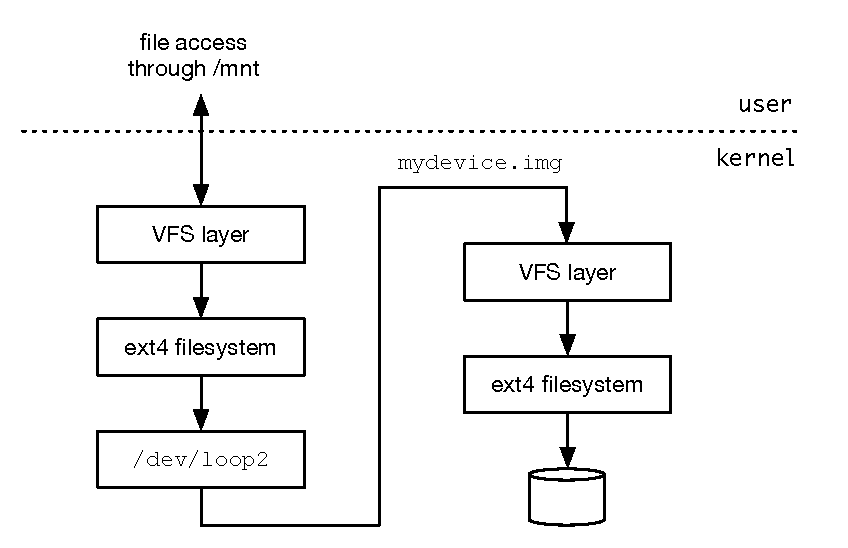
\includegraphics[scale=0.6]{figures/loopback.pdf}
	\centering
	\caption{Accessing a filesystem through a loop device}
	\label{fig:loopback}
\end{figure}

\noindent
xxx

\subsection{Demonstrating Loopback Devices}

This example shows how to create the loop device shown in figure \ref{fig:loopback}, create an ext4 filesystem on it, mount it to make it available for general use.

There are only a few simple steps needed to create a loopback device, add a filesystem and mount it to make it available. First of all, we created a 10 MB file:

\begin{lstlisting}
$ [*\bfseries dd if=/dev/zero of=~/mydevice.img bs=1024k count=10*]
5+0 records in
5+0 records out
5242880 bytes (5.2 MB, 5.0 MiB) copied, 0.00927079 s, 566 MB/s
\end{lstlisting}

\noindent
You can experiment with sizes. If you make it 5 MB, it will be too small for ext4 to add a journal but 10 MB is fine. The next step is to call \cf{losetup} to create a loopback device. The \cf{find} option locates the first available loop device and the \cf{show} option displays which loop device was assigned.

\begin{lstlisting}
$ [*\bfseries sudo losetup --find --show mydevice.img *]
/dev/loop2
\end{lstlisting}

\noindent
The device is accessible via \cf{/dev/loop2} so the next step is to make a filesystem on it, mount it and show space available:

\begin{lstlisting}
$ [*\bfseries sudo mkfs -t ext4 /dev/loop2*]
mke2fs 1.46.5 (30-Dec-2021)
Discarding device blocks: done                            
Creating filesystem with 2560 4k blocks and 2560 inodes

Allocating group tables: done                            
Writing inode tables: done                            
Creating journal (1024 blocks): done
Writing superblocks and filesystem accounting information: done
$ [*\bfseries sudo mount /dev/loop2 /mnt*]
mount: /mnt: /dev/loop2 already mounted on /mnt.
$ [*\bfseries df -h /mnt*]
Filesystem      Size  Used Avail Use% Mounted on
/dev/loop2      5.4M   24K  4.7M   1% /mnt
\end{lstlisting}

\noindent
It looks like, and will function like, any other filesystem. Once you no longer need the filesystem/device you can unmount it and call \cf{losetup} to detach the device. You can keep the file or remove it as needed.

\begin{lstlisting}
$ [*\bfseries sudo umount /mnt*]
$ [*\bfseries sudo losetup --detach /dev/loop2*]
\end{lstlisting}

\noindent
Once mounted, it looks like, and will function like, any other ext4 filesystem but with an additional overhead since there is now an ext4 filesystem on top of an ext4 file residing in another ext4 filesystem. 

Once you no longer need the filesystem/device you can unmount it and call \cf{losetup} to detach the device. You can keep the file or remove it as needed.

%%%%%%%%%%%%%%%%%%%%%%%%%%%%%%%%%%%%%%%%%%%%%%%%%%%%%%%%%%%%

\section{Client Caching With FS-Cache}

\textbf{is this the right place to cover this? I don't think so but come back later. Perhaps "miscelaneous topics"}

% https://www.kernel.org/doc/html/latest/filesystems/caching/fscache.html

FS-Cache is a persistent local cache introduced into Linux by Red Hat in 2001. It allows file systems to take data that has been retrieved from over the network and cache it on local disk. The goal is to help minimize network traffic for users on a client accessing data from a file system mounted over the network. NFS is one such example and an NFS mount option instructs the client to mount the NFS share with FS-Cache enabled.

Why not just utilize the page cache? What are the tradoffs? Data out of sync? Multiple users accessing the same files?


\begin{table}[h]
\begin{tabular}{ll}
\parbox[l]{0.6in}{
\includegraphics[scale=0.8]{figures/src-xref.pdf}} & \parbox[l]{4in}{\small{The FS-cache code can be found in \cf{fs/fscache}. There are only 2700 LOC.}}
\end{tabular}
\end{table}

\noindent
Figure \ref{fig:fscache} shows how FS-Cache works. \textbf{XXX---not sure this is correct. Come back once i figure it out}

\begin{figure}[h]
	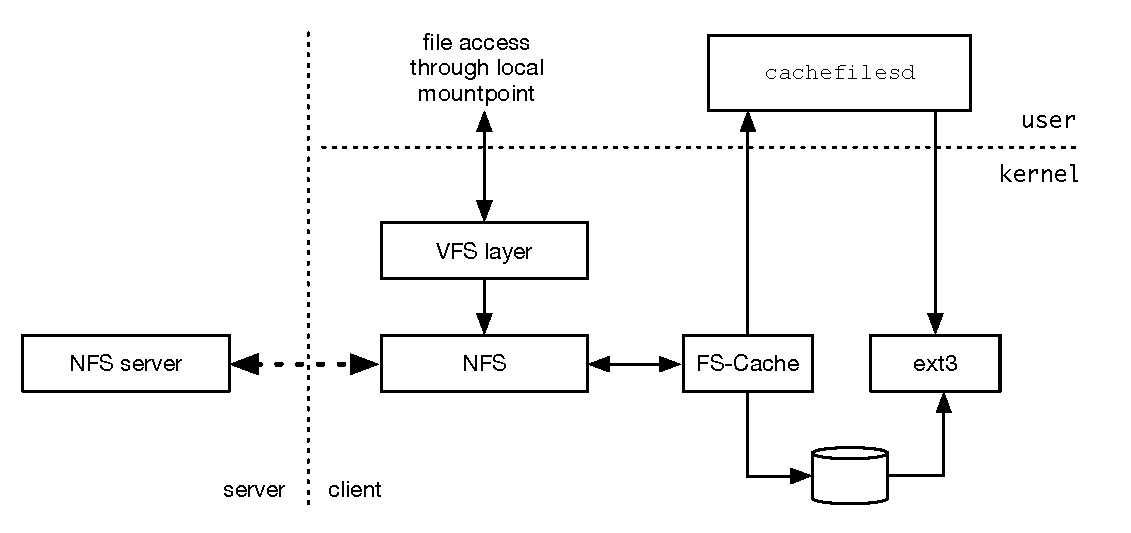
\includegraphics[scale=0.6]{figures/fscache.pdf}
	\centering
	\caption{Client caching with FS-Cache}
	\label{fig:fscache}
\end{figure}

\noindent
The goal of FS-Cache is that it should be as transparent as possible to the users and administrators of a system. In what circumstances is this transparency not achieved? \textbf{XXX---need to find out}.

FS-Cache does not alter the basic operation of a file system that works over the network - it merely provides that file system with a persistent place in which it can cache data. For instance, a client can still mount an NFS share whether or not FS-Cache is enabled. In addition, cached NFS can handle files that won't fit into the cache (whether individually or collectively) as files can be partially cached and do not have to be read completely up front. FS-Cache also hides all I/O errors that occur in the cache from the client file system driver.

Blah blah - NFS will not use FS-Cache unless explicitly stated when mounted as follows:

\begin{lstlisting}
# [*\bfseries mount nfs-share:/ /mount/point -o fsc}
\end{lstlisting}

\noindent
XXX - change args - try it first

%%%%%%%%%%%%%%%%%%%%%%%%%%%%%%%%%%%%%%%%%%%%%%%%%%%%%%%%%%%%

\section{Network Filesystems}

% https://developer.ibm.com/tutorials/l-network-filesystems/ - nice article

Simply put, a network file system allows a remote client to access a filesystem over a network in a similar way to a local file system. Developed over the course of forty years, Sun's NFS (Network Filesystem) has become the dominant network filesystem and has been ported to and ran on just about every operating system developed over that period of time. But NFS isn't the only network filesystem that Linux supports. NFS will be described soon but here are some other network filesystems that Linux supports:

% https://maxammann.org/posts/2022/01/linux-file-system-comparison/ - other nw fs

\begin{itemize}
	\item dav -- GVFS?
	\item davfs2 -- GVFS?
	\item sftp -- GVFS?
	\item SMB -- 
	\item CIFS -- 
	\item SSHFS -- a FUSE-based filesystem that runs on top of the SSH protocol, is accessible by non-root users and makes
		a remote directory visible through a local directory. 
\end{itemize}

\noindent
Which filesystem to use can depend on several factors - TBD - % https://serverfault.com/questions/196285/secure-network-filesystems-for-linux-what-are-people-doing

Section \ref{ssh-fs} shows an example of running SSHFS.

\subsection{NFS -- the Network File System}

NFS has been the most popular network filesystem for several decades now. It started at Sun Microsystems in 1984. The initial release (version 1) was primarily used in-house. This was followed by three major versions which will be described below.

The original paper \textit{The Sun Network Filesystem: Design, Implementation and Experience} can be found with the following link. It describes the goals of the project, how NFS utilized the new VFS/vnode architecture, architecture, design and implementation. The \textit{hard issues} are also described such as file locking.

\begin{table}[h]
\begin{tabular}{lcl}
\parbox[r]{0.5in}{
\includegraphics[scale=0.15]{figures/url.png}} & \parbox[l]{0.55in}{URL \arabic{urls} -- } & \parbox[l]{3in}{\cf{https://tinyurl.com/5f5tyakz}}
\end{tabular}
\end{table}
\stepcounter{urls}
% https://www.cs.ucf.edu/~eurip/papers/sandbergnfs.pdf

\noindent
Figure \ref{fig:nfs} shows the overall architecture of NFS as it was in the 1980s and also, as it is now in the Linux kernel today. There are actually two distinct filesystems, one on the client and one on the server. The client component appears as any other filesystem but takes VFS-level requests and communicates with the NFS server to fulfill them using NFS messages defined in the RFC standard. NFS was originally built on-top of UDP but for many years has primarily run over TCP/IP.

\begin{figure}[h]
	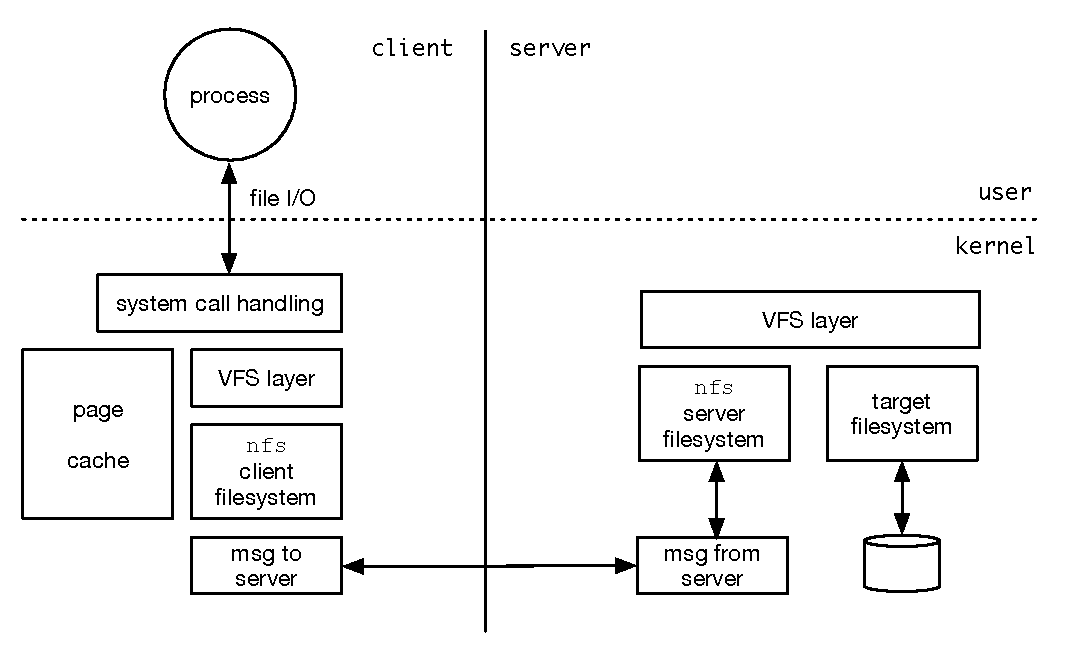
\includegraphics[scale=0.6]{figures/nfs.pdf}
	\centering
	\caption{NFS client and server}
	\label{fig:nfs}
\end{figure}

\noindent
NFS version 2 was defined in RFC 1094 and released in 1989, NFS v2 worked on top of UDP (User  Datagram Protocol) with the goal of being stateless. This meant that the NFS server was unaware of the clients accessing it therefore locking was implemented outside of the protocol. NFS v2 had a 2 GB file limit and poor performance due to synchronous writes. It would take  another few years before the Large File Summit (LFS) came into being with the goals of accessing files greater  than 2 GB. And 32-bit architectures were prevalent. NFS v2 was implemented on the new VFS/vnode architecture.

NFS version 3, defined in RFC 1813 and released in June 1995 had two main goals: add support for \textit{large files} (> 2 GB - 1) and improve performance. In addition to 64-bit file offsets, there were performance improvements in the following areas:

\begin{itemize}
	\item handling asynchronous writes on the server, to improve write performance.
	\item additional file attributes returned for many operations removing the need to keep making additional calls to retrieve them.
	\item a new \cf{READDIRPLUS} operation for which the server returned file handles and attributes along with file 
		names when scanning a directory.
\end{itemize}

\noindent
NFS was becoming very popular and interoperability annual testing occurred at \textit{Connectathon} events in 1986 where vendors would bring along their NFS client, server or both and informally test with each other. When I joined SCO in 1993, Lachmann Associates were providing our NFS and TCP/IP implementations. Around the time NFS v3 was being introduced, different operating system companies and NFS vendors such as Lachmann Associates, had already started to add NFS over TCP/IP where it offered better performance than UDP over WANs partly due to removing the 8 KB limit imposed by UDP.

For those interested in the history of the large file summit, details can be found here. Operating system and filesystem vendors spent a considerable amount of time in both attending these conferences and implementing support for large files.

\begin{table}[h]
\begin{tabular}{lcl}
\parbox[r]{0.5in}{
\includegraphics[scale=0.15]{figures/url.png}} & \parbox[l]{0.55in}{URL \arabic{urls} -- } & \parbox[l]{3in}{\cf{https://tinyurl.com/y4r8hep8}}
\end{tabular}
\end{table}
\stepcounter{urls}
% https://en.wikipedia.org/wiki/Large-file_support

\noindent
Following NFS v3, there was an extension introduced by Sun called WebNFS.

\begin{quote}WebNFS was an extension to NFSv2 and NFSv3 allowing it to function behind restrictive firewalls without the complexity of Portmap and MOUNT protocols. WebNFS had a fixed TCP/UDP port number (2049), and instead of requiring the client to contact the MOUNT RPC service to determine the initial file handle of every filesystem, it introduced the concept of a public filehandle (null for NFSv2, zero-length for NFSv3) which could be used as the starting point. Both of those changes have later been incorporated into NFSv4.\end{quote}

Sun Microsystems turned over the development of future NFS protocols to IETF (the Internet Engineering Task Force) and IETF was responsible for NFS versions 4 in 2000, 4.1 in 2010 and 4.2 in 2016.

NFS v4 introduced a stateful protocol and provided several security enhancements. TBD.

The NFS v4.1 protocol incorporated support for clustered server deployments. Under the pNFS extension, this provided support for scalable parallel access to files distributed among multiple servers. It also introduced a feature called \textit{session trunking}, also called NFS Multi-pathing ... introduced in VMware ESXi et al.

\begin{quote}
NFS version 4.2 (RFC 7862) was published in November 2016[9] with new features including: server-side clone and copy, application I/O advise, sparse files, space reservation, application data block (ADB), labeled NFS with sec\_label that accommodates any MAC security system, and two new operations for pNFS (LAYOUTERROR and LAYOUTSTATS).

One big advantage of NFSv4 over its predecessors is that only one UDP or TCP port, 2049, is used to run the service, which simplifies using the protocol across firewalls
\end{quote}

For more information about the history of NFS, Brent Callaghan's 1999 book \textit{NFS Illustrated}\cite{nfs}  is a good reference and covers all versions including WebNFS. Details about the NFS implementation in Linux can be found in section \ref{nfs-chapter}.

%%%%%%%%%%%%%%%%%%%%%%%%%%%%%%%%%%%%%%%%%%%%%%%%%%%%%%%%%%%%

\section{Backup / restore}\label{backups}

old days - dump(8)

dd vs FS backup (tar etc)?

xattrs etc

snapshots / freeze - usable - btrfs - anything that uses this stuff?

When I was at VERITAS and not long after we made our first port to Linux, we developed a feature that we called the File Change Long (FCL). One of the biggest problems with backup technology at the time was the time spent figuring out which files needed to be backed up. We also owned Netbackup which was the world's moist successful enterprise backup software. The time taken to scan the filesystem to determine which files needed to be backed up was extremely time consuming and the File Change Log could reduced that time dramatically.

Living in a world where servers are generally virtualized has changed the backup space dramatically with vendors such as Veeam backing up at the VM layer or even within the storage subsystem.

Having said that, this section explores the different backup and restore capabilities pro

\begin{itemize}
	\item rsync --
	\item tar / cpio --
	\item ReaR -- Relax and Recover 
	\item dump / restore--
	\item timeshift -- and btrfs support?
\end{itemize}

what works in the commercial space in Linux - open source vs ...

{\bfseries XXX---expand ...}

\subsection{Freezing and Thawing Filesystems}

% https://lwn.net/Articles/287435/

Freezing and thawing a filesystem was a features initially added to Linux to freeze an XFS filesystem when used with hardware RAID devices that support the creation of snapshots. This would involve a set of action such as:

\begin{lstlisting}
# [*\bfseries xfs\_freeze -f /xfs\_mnt*]

[*\itshape Take a snapshot of the file system ...*]

# [*\bfseries xfs\_freeze -u /xfs\_mnt*]
\end{lstlisting}

\noindent
This initial feature has now been extended to support 3xt3/4 and JFS in addition to XFS and is described in the \cf{fsfreeze(8)} manpage. There are two options:

\begin{enumerate}
	\item \cf{-freeze} / \cf{-f} -- freeze the filesystem from all future modifications. If there are any pending operations, they will be
		allowed to complete. Any subsequent calls to \cf{write(2)} (or similar system calls) will be suspended until an unfreeze
		request is made.
	\item \cf{-unfreeze} / \cf{-u} -- un-freeze the filesystem allowing operations to continue. If filesystem modifications  
		were blocked by call freeze call, they will be unblocked and allowed to complete.
\end{enumerate}

\noindent
A call to \cf{fsfreeze} is no necessary for device-mapper devices since device-mapper (and LVM) automatically freeze filesystems on the device when a snapshot creation is requested. For more details see the dmsetup(8) man page.

For further information, visit the following site:

\begin{table}[h]
\begin{tabular}{lcl}
\parbox[r]{0.5in}{
\includegraphics[scale=0.15]{figures/url.png}} & \parbox[l]{0.55in}{URL \arabic{urls}} & \parbox[l]{3in}{\cf{https://tinyurl.com/bkm7tyb3}}
\end{tabular}
\end{table}
\stepcounter{urls}
% https://docs.kernel.org/admin-guide/device-mapper/snapshot.html

\noindent
There are operations at the filesystem level in the kernel to support freeze / thaw which only a small number of filesystems support. These will be described in section \ref{freeze}.

Snapshots will be further described when the individual filesystems are discussed in detail - \textbf{section TBD}

%%%%%%%%%%%%%%%%%%%%%%%%%%%%%%%%%%%%%%%%%%%%%%%%%%%%%%%%%%%%

\section{Quotas}

File system quotas, which have been around since the early BSD UNIX days, are a mechanism to control the amount of disk space that can be consumed by specific users, by groups of users, or by a site-determined group of users called an \textit{admin set}. It's a feature that I haven't personally seen used a lot over my career but certainly has its place. I remember when I was working on VxFS at VERITAS, we spent considerable time on quotas but didn't use them ourselves. We opted for the old-fashioned way of running a script and emailing the filesystem team with who was using what space! This section shows how quotas can be used on Linux with an example of XXX.

xxx - blah

figure out who actually uses it and what filesystems?

There are three different types of quotas supported by Linux:

\begin{itemize}
	\item vfsold -- version 1 quotas.
	\item vfsv0 -- version 2 quotas.
	\item xfs -- the quota on XFS filesystems.
\end{itemize}

\noindent
To enforce vfsold and vfsv0 quota checking, you must turn it on using the \cf{quotaon} command. The newer version (vfsv0) provides a journald quota system, which means that a quota check is not needed during boot, something that can take considerable time.

There are both \textit{block limits} and \textit{file limits} for quotas. For both, quotas have both soft and hard limits. Generally speaking, a user is allowed to exceed the soft limit but not exceed the hard limit. However, there is a grace period for soft limits and once this grace period has expired the soft limit is treated like the hard limit.

To understand the different limits, here is output from the \cf{repquota(8)} command that will be explored in more detail in the next section:

\begin{lstlisting}
$ [*\bfseries sudo repquota -v /mnt*]
*** Report for user quotas on device /dev/sda1
Block grace time: 7days; Inode grace time: 7days
                        Block limits                File limits
User            used    soft    hard  grace    used  soft  hard  grace
----------------------------------------------------------------
root      --      20       0       0              2     0     0       
spate     +-   10252    5120   10240  6days       4    10    20       
ashley    --       0    5120   10240              0    10    20       
sam       --       0   10240   15360              0     5    10     
\end{lstlisting}

\noindent
The command shows block and file limits. User \cf{spate} has exceeded the block soft limit for which the grace period is 7 days.

\subsection{An Example of Using Filesystem Quotas on Ubuntu}

% https://www.digitalocean.com/community/tutorials/how-to-set-filesystem-quotas-on-ubuntu-18-04 - run on ubuntu
% https://linuxhint.com/disk_quota_ubuntu/
% btrfs and XFS have quota tools
% https://developer.ibm.com/tutorials/l-lpic1-v3-104-4/

To show how filesystem quotas are setup and used, this section shows a simple example of using user quotas on a Ubuntu system. To get started, the \cf{quota} tools package first needs to be installed as follows:

\begin{lstlisting}
$ [*\bfseries sudo apt install quota*]
\end{lstlisting}

\noindent 
To verify that the quota tools are installed correctly, run the following:

\begin{lstlisting}
$ [*\bfseries quota --version*]
Quota utilities version 4.06.
...
\end{lstlisting}

\noindent 
The goal here is to add user quotas for a filesystem on \cf{/dev/sda2}, to be mounted on \cf{/mnt}, to provide some limits for a specific set of users and show what happens when these limits are exceeded.

The first step is to make an ext4 filesystem and enable user quotas:

\begin{lstlisting}
$ [*\bfseries sudo mkfs.ext4 -Equotatype=usrquota /dev/sda1*]
mke2fs 1.46.5 (30-Dec-2021)
Discarding device blocks: done                            
Creating filesystem with 261888 4k blocks and 65536 inodes
Filesystem UUID: 68b55c65-22ee-454d-8a60-1b99ed1c861c
Superblock backups stored on blocks: 
	32768, 98304, 163840, 229376

Allocating group tables: done                            
Writing inode tables: done                            
Creating journal (4096 blocks): done
Writing superblocks and filesystem accounting information: done
\end{lstlisting}

\noindent 
Mount the filesystem specifying the usrquota option: \textbf{XXX---when should quotaon be run?}

\begin{lstlisting}
$ [*\bfseries sudo mount -ousrquota /dev/sda1 /mnt*]
\end{lstlisting}

\noindent 
Check to make sure that quotas are enabled for this mountpoint:

\begin{lstlisting}
$ [*\bfseries mount | grep sda1*]
/dev/sda1 on /mnt type ext4 (rw,relatime,quota,usrquota)
\end{lstlisting}

\noindent 
Run quotacheck which can scan a filesystem for disk usage, create, check 
and repair quota files. Without any arguments it will create the file aquota.user in the root directory.

\begin{lstlisting}
$ [*\bfseries sudo quotacheck /mnt*]
22.10-target$ ls /mnt
aquota.user  lost+found/
\end{lstlisting}

\noindent 
The setquota command can be used to set quota limits. The arguments are:

\begin{lstlisting}
$ [*\bfseries sudo setquota -u [username] [soft disk limit] [hard disk limit] *]
  [soft inode limit] [hard inode limit]  [partition]
\end{lstlisting}

\noindent 
To set limits for user ashley:

\begin{lstlisting}
$ [*\bfseries sudo setquota -u ashley 5M 10M 10 20 /mnt*]
$ [*\bfseries sudo setquota -u sam 10M 15M 5 10 /mnt*]
\end{lstlisting}

\noindent
xxx

\begin{lstlisting}
$ [*\bfseries sudo quota -vs ashley *]
Disk quotas for user ashley (uid 1001): 
     Filesystem   space   quota   limit   grace   files   quota   limit   grace
/dev/mapper/ubuntu--vg-ubuntu--lv
                    16K      0K      0K               4       0       0        
      /dev/sda1      0K   5120K  10240K               0      10      20 
\end{lstlisting}

\noindent 
To report usage the \cf{repquota(8)} command can be used as follows:

\begin{lstlisting}
$ [*\bfseries sudo repquota -s /mnt*]
*** Report for user quotas on device /dev/sda1
Block grace time: 7days; Inode grace time: 7days
                        Space limits                File limits
User            used    soft    hard  grace    used  soft  hard  grace
----------------------------------------------------------------------
root      --     20K      0K      0K              2     0     0  
\end{lstlisting}

\noindent 
If users have not yet created any files, nothing will be displayed. But this displays more:

\begin{lstlisting}
$ [*\bfseries sudo repquota -v /mnt*]
*** Report for user quotas on device /dev/sda1
Block grace time: 7days; Inode grace time: 7days
                        Block limits                File limits
User            used    soft    hard  grace    used  soft  hard  grace
----------------------------------------------------------------------
root      --      20       0       0              2     0     0       
spate     --       0    5120   10240              0    10    20       
ashley    --       0    5120   10240              0    10    20       
sam       --       0   10240   15360              0     5    10       

Statistics:
Total blocks: 7
Data blocks: 1
Entries: 4
Used average: 4.000000
\end{lstlisting}

\noindent 
but spate has created files and nothing is being shown. If I run:

\begin{lstlisting}
$ [*\bfseries sudo quotacheck /mnt*]
\end{lstlisting}

\noindent 
again I can then see info:

\begin{lstlisting}
$ [*\bfseries sudo repquota -v /mnt*]
*** Report for user quotas on device /dev/sda1
Block grace time: 7days; Inode grace time: 7days
                        Block limits                File limits
User            used    soft    hard  grace    used  soft  hard  grace
----------------------------------------------------------------------
root      --      20       0       0              2     0     0       
spate     +-   10252    5120   10240  7days       4    10    20       
ashley    --       0    5120   10240              0    10    20       
sam       --       0   10240   15360              0     5    10       

Statistics:
Total blocks: 7
Data blocks: 1
Entries: 4
Used average: 4.000000
\end{lstlisting}

\noindent 
they say that quotacheck should be run without users accessing the filesystem.


%%%%%%%%%%%%%%%%%%%%%%%%%%%%%%%%%%%%%%%%%%%%%%%%%%%%%%%%%%%%

\section{Swap space}\label{swap}

Swap space has traditionally been an area on disk used to temporarily write memory pages, thus freeing them up for use by other processes or even the same process depending on memory usage. This creates the illusion of having more physical memory than is actually available although it comes at a cost, namely performance.

Traditionally, swap space has been to a raw device, a feature that Linux offers. Some versions of UNIX later (from SVR4 onwards) included a swap filesystem. Swapfs was unusual in that it used physical memory for the swap space, but also required physical swap space on a disk.

Linux supports traditional swap devices in addition to the ability to swap to a file within a filesystem with use of the \cf{mkswap(8)} and \cf{swapon(8)} commands.

Rules about the amount of swap space being needed has been debated for years but really depends on the application load that is being run. If your mission critical database is constantly paging to/from swap, you're in trouble. The rule of thumb used to be 2x the amount of RAM in the system but with today's much larger RAM configurations or suspending a laptop, this general rule of thumb may not always make less sense. The following article gives a good guide as to how much swap space may be needed.

\begin{table}[h]
\begin{tabular}{lcl}
\parbox[r]{0.5in}{
\includegraphics[scale=0.15]{figures/url.png}} & \parbox[l]{0.55in}{URL \arabic{urls}} & \parbox[l]{3in}{\cf{https://tinyurl.com/mryahu3m}}
\end{tabular}
\end{table}
\stepcounter{urls}
% https://opensource.com/article/18/9/swap-space-linux-systems

\noindent
The \cf{free(1)} command can be used to display amount of free and used memory in the system. In this example, on the VM I am using where I am doing nothing but configure swap devices at the time of writing, there is little activity. Thus the RAM is only being partially used and no swap space is being used.

\begin{lstlisting}
# [*\bfseries free*]
               total        used        free  shared  buff/cache   available
Mem:         4006060      251732     1004024    5368     2750304     3557676
Swap:         262140           0      262140
\end{lstlisting}

\noindent
To illustrate how swapping to a file on a filesystem works,  the following example makes use of the \cf{mkswap(8)} and \cf{swapon(8)} commands to create a swap file.

The first step is to create a file which will be used as a swap device. In this example, the file is \cf{/swapfile} and it is 256 MB in size:

\begin{lstlisting}
# [*\bfseries dd if=/dev/zero of=/swapfile1 bs=1M count=256*]
262144+0 records in
262144+0 records out
268435456 bytes (268 MB, 256 MiB) copied, 0.384721 s, 698 MB/s
\end{lstlisting}

\noindent
Next, the permissions should be changed so that it's readable and writable by root but nobody else. You do not want regular users being able to read from this file as it may contain sensitive data.

\begin{lstlisting}
# [*\bfseries chmod 0600 /swapfile*]
# [*\bfseries ls -l /swapfile *]
-rw------- 1 root root 268435456 May  3 16:13 /swapfile
\end{lstlisting}

\noindent
The \cf{mkswap(8)} command is then run to set up a Linux swap area on the file.

\begin{lstlisting}
# [*\bfseries mkswap /swapfile*]
Setting up swapspace version 1, size = 256 MiB (268431360 bytes)
no label, UUID=043d78c9-295e-4a23-895f-c0ed6e4f51b5
\end{lstlisting}

\noindent
The second to last step is to activate the swap space as follows:

\begin{lstlisting}
# [*\bfseries swapon /swapfile*]
# [*\bfseries swapon*]
NAME      TYPE SIZE USED PRIO
/swapfile file 256M   0B   -2
\end{lstlisting}

\noindent
Lastly, \cf{/etc/fstab} should be modified to enable the swap file automatically on boot. An entry in \cf{/etc/fstab} will look like:

\begin{lstlisting}
/swapfile          swap            swap    defaults        0 0
\end{lstlisting}

\noindent
As mentioned above, this topic is skirting the area of filesystem access since the the filesystem does not see this file as being anything special. The only other thing to point out is that the space in the file could be quite fragmented so if a file with an extent of the size of the swap device could be created, that would help with performance. More importantly would be to have the block size of the filesystem be the same as the page size so page-sized writes do not get split up and written to different locations on disk.

%%%%%%%%%%%%%%%%%%%%%%%%%%%%%%%%%%%%%%%%%%%%%%%%%%%%%%%%%%%%

\section{The Boot Process and Run Levels}

As seen earlier and by running \cf{mount(1)} there are 34 filesystems mounted on a simple Ubuntu VM. When do these filesystems get mounted or unmounted? Certainly by the time the system is up they are there and accessible. When to mount them is determine as part of boot process.

boot to single user and show what's mounted

apart from ramfs, say what?

Here are the 6 different run levels. The run level number is on the left.

\begin{enumerate}
	\item System halt i.e the system can be safely powered off with no activity.
	\item Single user mode.
	\item Multiple user mode with no NFS(network file system).
	\item Multiple user mode under the command line interface and not under the graphical user interface.
	\item User-definable.
	\item Multiple user mode under GUI (graphical user interface) and this is the standard runlevel for most of the LINUX based systems.
	\item Reboot which is used to restart the system.
\end{enumerate}

\noindent
The \cf{telinit(8)} command can be used to change the run level.

\subsection{Run Level Scipts}

At each run level, init (???) will execute a set of scripts. ... this is a lot more complex than it used to be. History:

below is cut n paste so needs rewording

\begin{itemize}
	\item System V init -- this is the traditional init --  \textbf{not used anymore?}
	\item Upstart init, used by older Ubuntu and some RHEL (Red Hat) and older Fedora versions
	\item systemd init, used by modern Fedora, Ubuntu, Debian, RHEL, SUSE versions
\end{itemize}

\noindent
The \textit{systemd init} is described by the \cf{systemd(1)} manpage. 

user@.service(5) and a whole host of others

everything is in /etc/init.d and /etc/rcX.d/* contains symlinks to files in /etc/init.d

run level scripts are in /etc/rcX.d

\begin{lstlisting}
$ [*\bfseries ls /etc/rc*]
rc0.d/ rc1.d/ rc2.d/ rc3.d/ rc4.d/ rc5.d/ rc6.d/ rcS.d/ 
\end{lstlisting}

\noindent
For example, here are the contents of \cf{rc3.d}:

\begin{lstlisting}
K01sysstat -> ../init.d/sysstat
S01apport -> ../init.d/apport
S01console-setup.sh -> ../init.d/console-setup.sh
S01cron -> ../init.d/cron
S01dbus -> ../init.d/dbus
S01grub-common -> ../init.d/grub-common
S01irqbalance -> ../init.d/irqbalance
S01lvm2-lvmpolld -> ../init.d/lvm2-lvmpolld
S01multipath-tools -> ../init.d/multipath-tools
S01open-vm-tools -> ../init.d/open-vm-tools
S01plymouth -> ../init.d/plymouth
S01rsync -> ../init.d/rsync
S01ssh -> ../init.d/ssh
S01unattended-upgrades -> ../init.d/unattended-upgrades
S01uuidd -> ../init.d/uuidd
\end{lstlisting}

\noindent
Each file is a symlink to a script in \cf{/etc/init.d}.

XXX still don't know when filesystems are mounted!!!

The meaning of each run level is as follows:

\begin{itemize}
	\item [0] -- Shut down (or halt) the system.
	\item [s] -- Single-user-mode; usually aliased as 's' or 'S'.
	\item [2] -- Multiuser mode without networking.
	\item [3] -- Multiuser mode with networking.
	\item [5] -- Multiuser mode with networking and the X Window System.
	\item [6] -- Reboot the system.
\end{itemize}

\noindent
Most people are unlikely to need to deal with run levels. With personal VMs/systems it's usual just to start, pause, shutdown or reboot. Installing software that needs to be started when the system boots and shutdown cleanly on reboot or shutdown will require knowledge of how \cf{systemd(1)} works. 

%%%%%%%%%%%%%%%%%%%%%%%%%%%%%%%%%%%%%%%%%%%%%%%%%%%%%%%%%%%%

\section{Conclusion}

This chapter presented many topics related to filesystems from disk partitioning to mounting different filesystems, pseudo filesystems, network filesystems and how the different main Linux filesystems compare in terms of features and performance.. 

Now that we've described all the file/filesystem-related programming interfaces and this chapter has covered filesystem-level topics, it's time to start exploring how filesystems are implemented in the Linux kernel. The next chapter starts to explore the Linux source code, providing tools for navigating around very large code base and describing where the filesystem-related code is. Subsequent chapters then start to dig deeper into kernel operations culminating in developing of a kernel-based filesystem and multiple user-space filesystems.

